\documentclass{ctexart}
\usepackage{amsmath}
\usepackage{booktabs}
\usepackage{listings}
\usepackage{graphicx}
\begin{document}
\lstset{language=fortran}
\title{计算物理学第一次作业}
\author{谭淞宸 1700011706\thanks{tansongchen@pku.edu.cn}}
\date{2019.04}
\newcommand{\f}{\mathrm{d}}
\maketitle
\paragraph{作业摘要}
本文中,所有程序均使用 Fortran 90 编写,并在 Mac OS 10.14.3 的终端使用 gcc 8.3.0 中的 gfortran 模块编译。阅读提示:
\begin{enumerate}
	\item 第一题至第七题每题在 code 文件夹下设有一个文件夹(如 \verb|1/|);
	\item 第一题有两个源代码文件 \verb|1_1.f90| 和 \verb|1_2.f90| ;第七题有三个源代码文件 \verb|7_1.f90|, \verb|7_2.f90| 和 \verb|7_3.f90|;其余各题均有且仅有一个代码文件 \verb|n.f90|;每个代码对应一个无后缀的可执行文件。
	\item 第一题的两个代码文件分别对应输入文件 \verb|1_1_input.txt| 和 \verb|1_2_input.txt|,其余各题均无输入文件,也不需要在执行过程中输入;
	\item 所有代码文件均对应输出文件 \verb|<可执行文件名>_output.txt|;
	\item 如需编译,请在命令行下转到相应目录并输入(例如第 7 题第 2 小题) \verb|gfortran 7_2.f90 -o 7_2|,这样会生成相应的无后缀可执行文件;继续输入 \verb|./7_2| 执行该文件;不推荐双击执行该文件,因为这可能导致工作目录(CWD)的错判进而无法在正确的位置读入和输出文件;
	\item 对于题目中涉及可变参数的情况,所有代码中均自动遍历所有参数,因此只需要运行 1 次;结果输出到屏幕并保存到输出文件(提交时已经运行过并生成了相应的输出文件);
	\item 为使得阅读方便,本文件中的源代码加入了一些 Fortran 语言中的断行符 \verb|&|,请以代码文件中的为准。
\end{enumerate}
\newpage
\section{十进制数与双精度浮点数编码的相互转换}
\subsection{问题描述}
实现任意十进制数与其规范化的二进制双精度浮点数编码间的相互转换。
\subsection{解答思路}
\subsubsection{十进制数转双精度浮点数编码}
分两种情况讨论。按 IEEE-754 标准,若最高位不全为 0 且不全为 1,则为「规约数」,此时按如下思路转为编码:
\begin{enumerate}
    \item 确定符号位,并取绝对值;
    \item 如果绝对值大于等于 2,则不断除以 2 直至绝对值位于 [1,2) 内,指数部分从 1023 开始逐次增 1;
    \item 如果绝对值小于 1,则不断乘以 2 直至绝对值位于 [1,2) 内,指数部分从 1023 开始逐次减 1;
    \item 得到一个 [1,2) 内的数,将其减去 1,然后不断乘以 2 并判断得到的结果是否大于 1,如果是将相应小数位置 1,否则置 0;
    \item 将符号、指数、小数三部分合起来即可。
\end{enumerate}
若为「非规约数」,有如下几种情况:
\begin{enumerate}
    \item 输入的绝对值大于 $2^{1024}$ 即归为正负无穷大;
    \item 输入无法识别为数字即归为 NaN;
    \item 输入的绝对值小于 $2^{-1022}$,可以将其乘以 $2^{1022}$ 后归于规格化的第 4 步继续处理。
\end{enumerate}
\subsubsection{双精度浮点数编码转十进制数}
首先判断是否属于上述非规约数的一种,进行特别转换。如果不属于,按如下思路转为十进制数:
\begin{enumerate}
    \item 确定符号位;
    \item 指数初值为 -1023,按第 2 到 12 位的二进制编码依次增加;
    \item 小数初值为 1.0(高位为 0 的非规约数也参与此步转换,且初值为 0.0),按第 13 到 64 位的二进制编码依次增加;
    \item 将所得的三部分相乘即可。
\end{enumerate}
\subsection{算法描述}
\subsubsection{十进制数转双精度浮点数编码}
\begin{lstlisting}
输入:a
输出:code(64)

read a
! 处理符号,并覆盖为绝对值
if (a < 0)
    code(1) = 1
    a = abs(a)
! 处理高位全为 1 的非规约数(无穷大)
if (a = infinity)
    code(2:12) = 1
else
! 处理高位全为 0 的非规约数,乘以一个规约化因子
    if (a < min_limit) a = a * 2**1022
    ! 处理规约数
    else
    ! 处理规约数的指数部分
    ! 并让大数除 2、小数乘 2 直至落入范围
        code(2:12) = 1023 + [log_2(a)]
        a * 2.0 or / 2.0 → [1, 2)
        a = a - 1
        ! 处理小数
        code(13:64) = a 的小数部分
write code
\end{lstlisting}
\subsubsection{双精度浮点数编码转十进制数}
\begin{lstlisting}
输入:code(64)
输出:a

read code
! 非规约数,高位全为 1
if (all(code(2:12) == 1)) then
    ! 低位有 1,则不是数
    if (any(code(13:64) == 1)) write 'NaN'
    ! 低位无 1,根据符号确定正负无穷大
    else write '+Infinity' or '-Infinity'
else
    ! 生成符号
    if (code(1) == 1) sign = -1
    ! 非规约数,高位全为 0
    if (all(code(2:12) == 0)) then
        decimal = 0.0, exponent = -1022
    ! 剩下的都是规约数
    else
        exponent ← code(2:12)
    ! 小数
    decimal ← code(13:54)
    ! 乘起来
    factor = 2 ** exponent
    a = sign * factor * decimal
write a
\end{lstlisting}
\subsection{计算结果与讨论}
选取几个有代表性的数放入输入文件,程序从相应的输入文件读入数据,转换后显示在屏幕上并保存到相应的输出文件。
\begin{figure}[h]
\centering
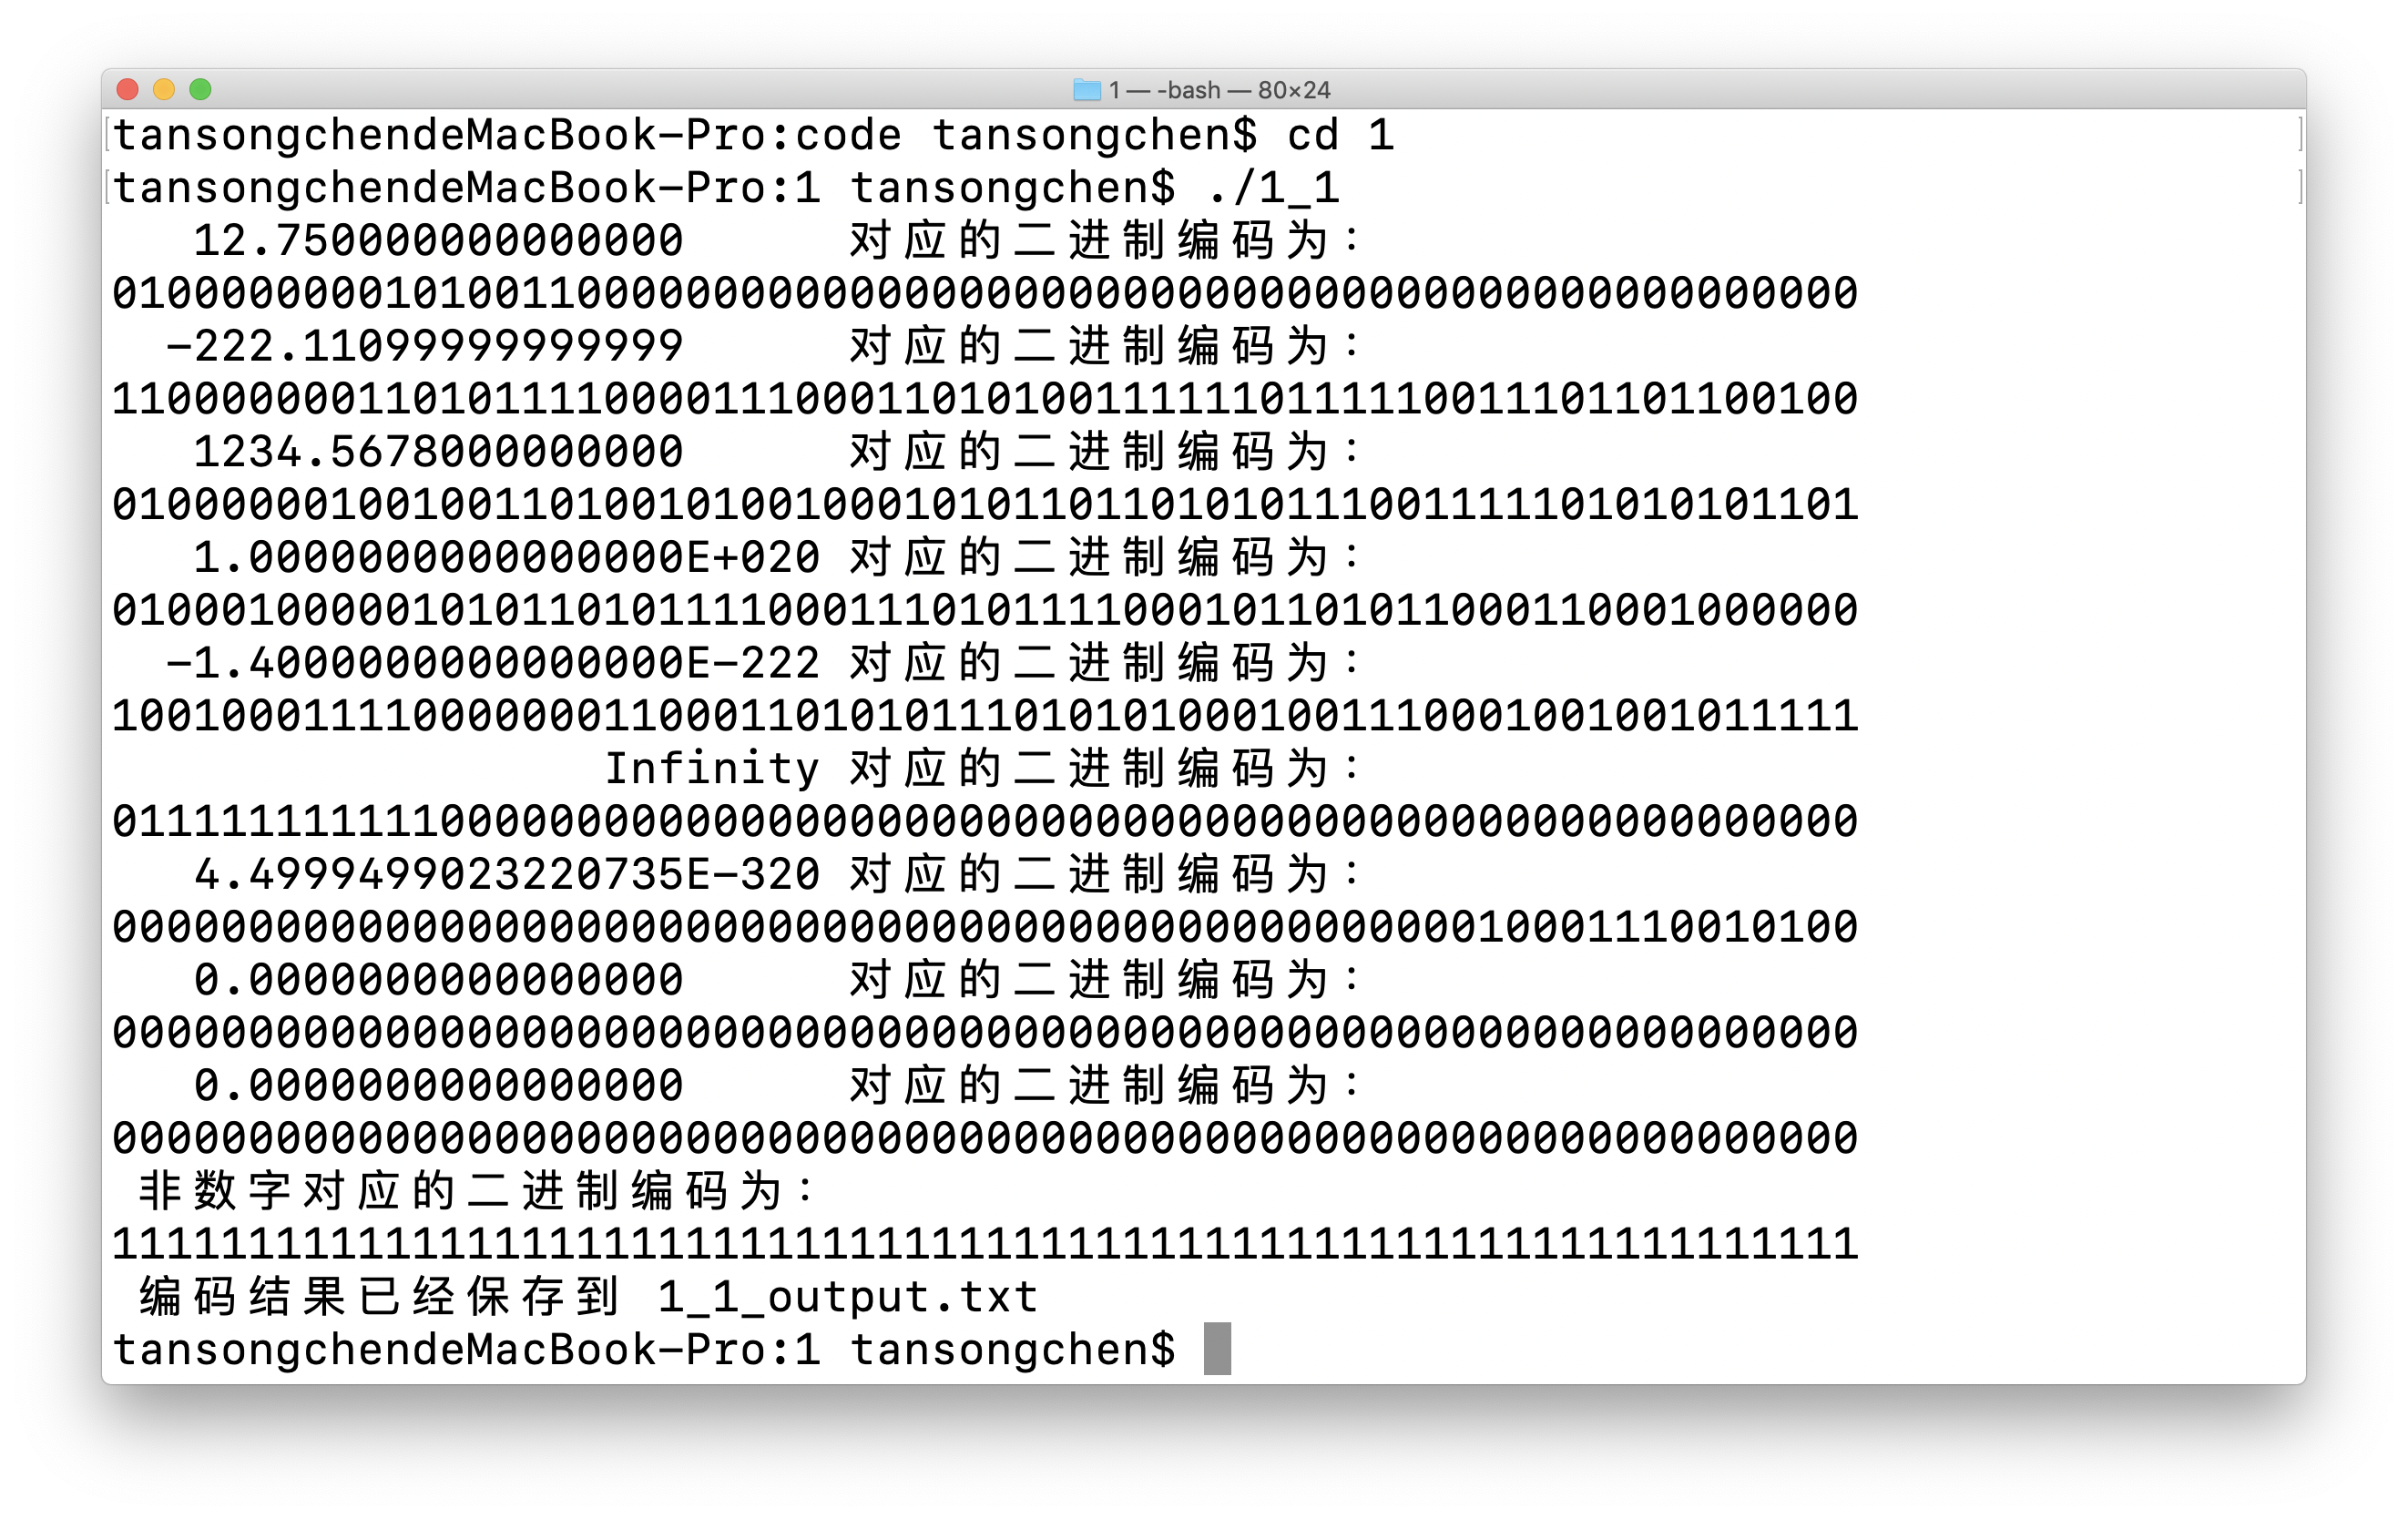
\includegraphics[scale = 0.3]{1.png}
\caption{十进制数转双精度浮点数编码}
\end{figure}
\begin{figure}[h]
\centering
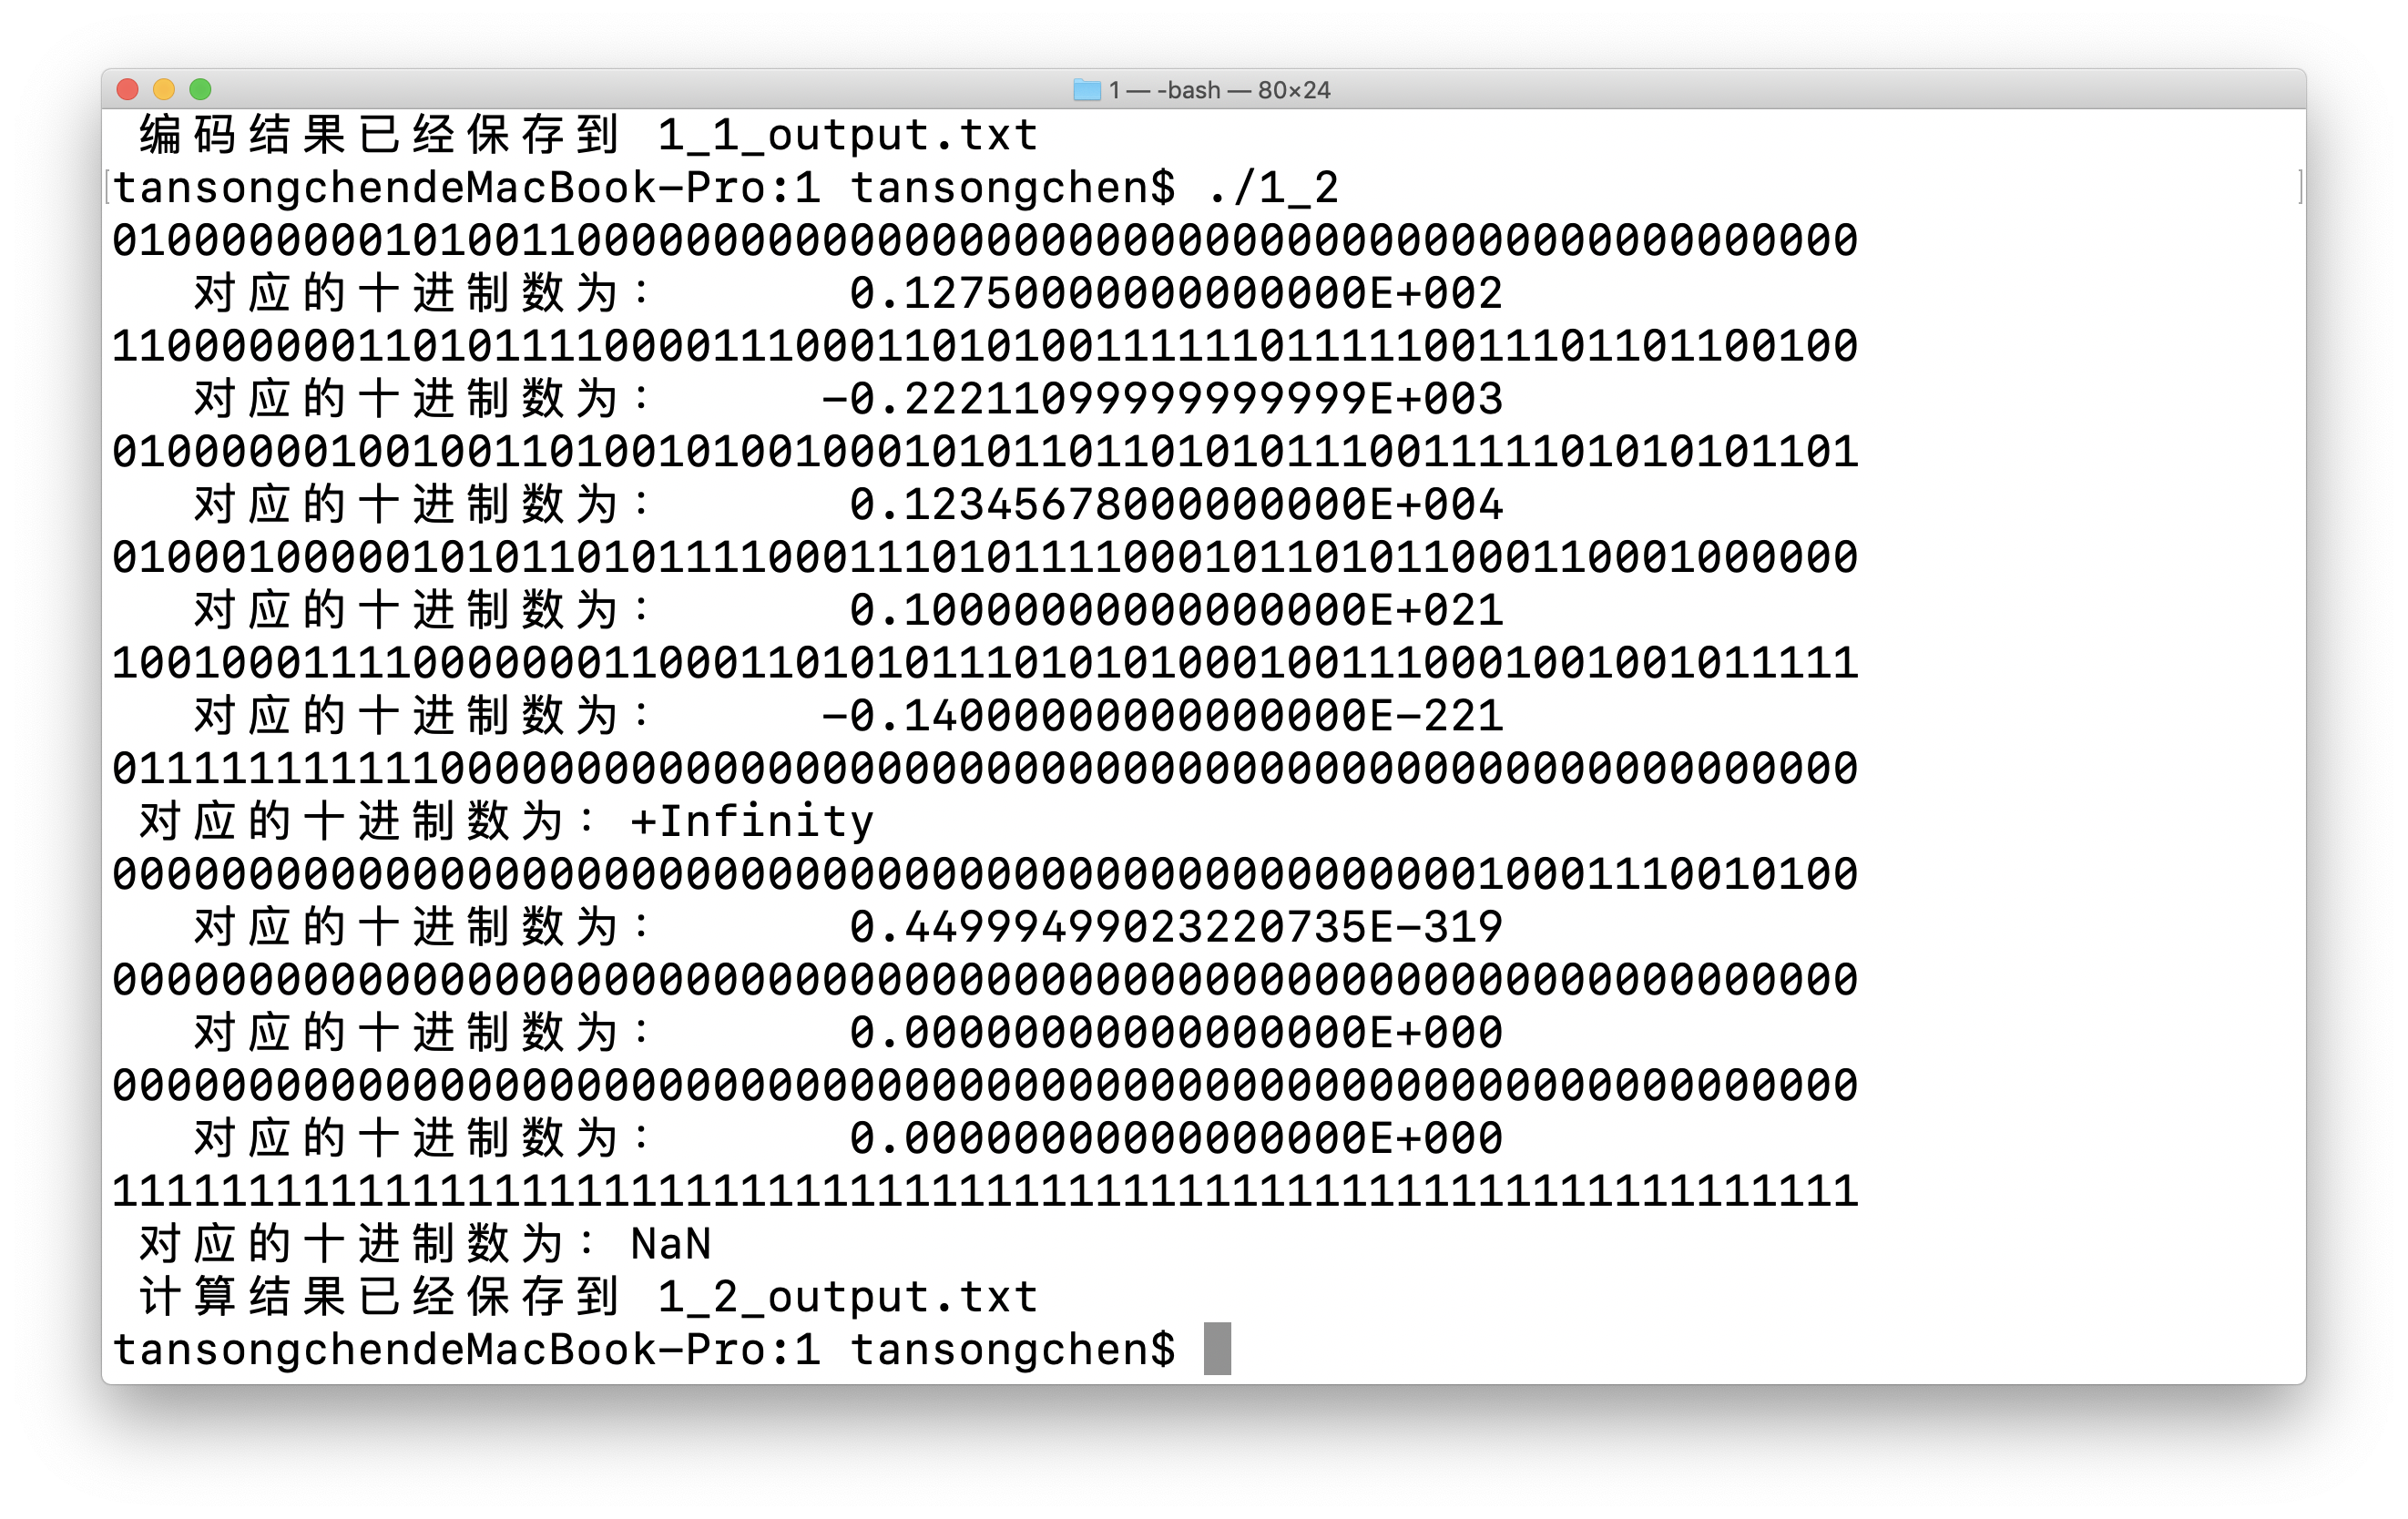
\includegraphics[scale = 0.3]{2.png}
\caption{双精度浮点数编码转十进制数}
\end{figure}
\subsection{源代码}
\subsubsection{十进制数转双精度浮点数编码}
\begin{lstlisting}
program project1_1
	real*8, parameter :: binary = 2.0 ! 定义进制
	real*8, parameter :: max = binary ** 1024 ! 规格数上限
	real*8, parameter :: min = binary ** (-1022) ! 规格数下限
	integer :: code(64) = 0 ! 用数组存编码
	real*8 a, a_original ! 待转换的数
	integer i
	integer :: exponent = 1023 ! 指数偏移值

	open (10, file = '1_1_input.txt')
	open (11, file = '1_1_output.txt')
	do while (.true.)
		code = 0
		exponent = 1023
		! a_original 用来保存原始的数
		read (10, *, iostat = i) a_original
		if (i < 0) exit
		if (i > 0) then
			code = 1
			write (*, *) '非数字对应的二进制编码为:'
			write (*, '(64I1)') code
			write (11, '(64I1)') code
			cycle
		end if
		! 处理符号
		if (a_original < 0) code(1) = 1
		! 从这里开始,a 用来进行各种操作
		a = abs(a_original)
		! 处理非规约数
		! 第一种情况:如果绝对值上溢,则设为无穷大
		if (a == max) then
			code(2:12) = 1
			write (*, *) a_original, '对应的二进制编码为:'
			write (*, '(64I1)') code
			write (11, '(64I1)') code
			cycle
		end if
		! 第二种情况:如果低于最小规约数,乘以一个因子
		if (a < min) then
			a = a * 2**1022
		! 处理规约数
		else
			! 正常数的指数部分,大数除 2,小数乘 2
			do while (a >= 2)
				a = a / 2.0
				exponent = exponent + 1
			end do
			do while (a < 1)
				a = a * 2.0
				exponent = exponent - 1
			end do
			! 得到指数,将十进制转化为二进制
			do i = 12, 2, -1
				code(i) = mod(exponent, 2)
				exponent = exponent / 2
			end do
			! 小数部分需要减去 1
			a = a - 1
		end if
		! 处理小数,每一步乘 2
		! 如果大于 1 则二进制位为 1,否则为 0
		do i = 13, 64
			a = a * 2
			code(i) = int(a)
			if (a >= 1) a = a - 1
		end do
		write (*, *) a_original, '对应的二进制编码为:'
		write (*, '(64I1)') code
		write (11, '(64I1)') code
	end do
	write (*, *) '编码结果已经保存到 1_1_output.txt'
end program
\end{lstlisting}
\subsubsection{双精度浮点数编码转十进制数}
\begin{lstlisting}
program project1_2
	real*8, parameter :: binary = 2.0
	real*8 factor
	integer :: code(64) = 0
	real*8 a
	integer i
	integer :: sign = 1, exponent = -1023
	real*8 :: decimal = 1.0, unit = 1.0

	open (10, file = '1_2_input.txt')
	open (11, file = '1_2_output.txt')
	do while (.true.)
		code = 0
		sign = 1
		exponent = -1023
		decimal = 1.0
		unit = 1.0
		! a_original 用来保存原始的数
		read (10, '(64I1)', iostat = i) code
		if (i < 0) exit
		write (*, '(64I1)') code
		if (i > 0) then
			write (*, *) '不是有效的二进制编码'
			cycle
		end if
		! 非规约数,高位全为 1
		if (all(code(2:12) == 1)) then
			! 低位有 1,则不是数
			if (any(code(13:64) == 1)) then
				write(*, *) '对应的十进制数为:NaN'
			! 低位无 1,则为无穷大
			else
				if (code(1) == 0) then 
					write(*, *) &
					'对应的十进制数为:+Infinity'
				else
					write(*, *) &
					'对应的十进制数为:-Infinity'
				end if
			end if
			cycle
		end if
		! 处理符号
		if (code(1) == 1) sign = -1
		! 非规约数,高位全为 0
		if (all(code(2:12) == 0)) then
			decimal = 0.0
			exponent = -1022
		! 规约数
		else
			! 指数部分
			do i = 2, 12
				exponent = exponent + &
				2**(12 - i) * code(i)
			end do
		end if
		! 小数部分,每一步加上该位上的一个单位或不加
		do i = 13, 64
			unit = unit / 2.0
			decimal = decimal + unit * code(i)
		end do
		! 相乘
		factor = binary ** exponent
		a = sign * factor * decimal
		write (*, '(A30, E30.17E3)') '对应的十进制数为:', a
		write (11, *) a
	end do
	write (*, *) '计算结果已经保存到 1_2_output.txt'
end program
\end{lstlisting}
\newpage
\section{Gauss 求积公式}
\subsection{问题描述}
构造如下三种非标准权函数的 Gauss 求积公式中的求积系数和节点:

\[
\int_0^1 \sqrt xf(x)\f x\approx A_0f(x_0)+A_1f(x_1)
\]
\[
\int_0^1 \sqrt xf(x)\f x\approx B_0f(x_0')+B_1f(x_1')+B_2f(x_2')
\]
\[
\int_{-1}^1(1+x^2)f(x)\f x\approx C_0f(x_0'')+C_1f(x_1'')
\]

\subsection{解答思路}
首先考虑前两个以 $\sqrt x$ 为权的求积公式。

根据求积节点构造的定理,节点是次数分别为 2 和 3 的多项式的根,这些多项式与任何次数低于自身的多项式在 $[0,1]$ 上带权 $\sqrt x$ 正交。换言之,我们需要在四维多项式线性空间中构造一组带权 $\sqrt x$ 正交基,记作 $Q_n(x)$。为此,我们选取一组基 $\{1,x,x^2,x^3\}$,并进行 Schmidt 正交化,约定内积算符 $(f(x),g(x))=\int_0^1\sqrt xf(x)g(x)\f x$:

\[
Q_0(x)=1
\]
\[
Q_1(x)=x-\frac{(x,Q_0)}{(Q_0,Q_0)}Q_0=x-\frac35
\]
\[
Q_2(x)=x^2-\frac{(x^2,Q_1)}{(Q_1,Q_1)}Q_1-\frac{(x^2,Q_0)}{(Q_0,Q_0)}Q_0=x^2-\frac{10}9x+\frac5{21}
\]
\[
Q_3(x)=x^3-\frac{(x^3,Q_2)}{(Q_2,Q_2)}Q_2-\frac{(x^3,Q_1)}{(Q_1,Q_1)}Q_1-\frac{(x^3,Q_0)}{(Q_0,Q_0)}Q_0=x^3-\frac{21}{13}x^2+\frac{105}{143}x-\frac{35}{429}
\]

$Q_2$ 的根为 $x_0,x_1$,可以利用求积公式具有 0 和 1 次代数精度的条件求出求积系数(尽管该公式具有 3 次代数精度):
\[
\begin{cases}
\int_0^1 \sqrt x\cdot 1\f x=\frac23=A_0+A_1\\
\int_0^1 \sqrt x\cdot x\f x=\frac25=A_0x_0+A_1x_1
\end{cases}
\]

$Q_3$ 的根为 $x_0',x_1',x_2'$,可以利用求积公式具有 0, 1 和 2 次代数精度的条件求出求积系数:
\[
\begin{cases}
\int_0^1 \sqrt x\cdot 1\f x=\frac23=B_0+B_1+B_2\\
\int_0^1 \sqrt x\cdot x\f x=\frac25=B_0x_0'+B_1x_1'+B_2x_2'\\
\int_0^1 \sqrt x\cdot x^2\f x=\frac27=B_0x_0'^2+B_1x_1'^2+B_2x_2'^2
\end{cases}
\]

同理,对于权 $1+x^2$,我们需要在三维多项式线性空间中构造一组带权 $1+x^2$ 正交基,记作 $R_n(x)$。为此,我们选取一组基 $\{1,x,x^2\}$,并进行 Schmidt 正交化,约定内积算符 $[f(x),g(x)]=\int_{-1}^1(1+x^2)f(x)g(x)\f x$(注意到当奇函数在对称区间上积分为 0 将简化下述计算):

\[
R_0(x)=1
\]
\[
R_1(x)=x-\frac{[x,R_0]}{[R_0,R_0]}R_0=x
\]
\[
R_2(x)=x^2-\frac{[x^2,R_1]}{[R_1,R_1]}R_1-\frac{[x^2,R_0]}{[R_0,R_0]}R_0=x^2-\frac25
\]

$R_2$ 的根为 $x_0''=-\sqrt{2/5},x_1''=-\sqrt{2/5}$,可以利用求积公式具有 0 和 1 次代数精度的条件求出求积系数:
\[
\begin{cases}
\int_{-1}^1 (1+x^2)\cdot 1\f x=\frac83=C_0+C_1\\
\int_{-1}^1 (1+x^2)\cdot x\f x=0=C_0z_0+C_1z_1
\end{cases}
\]

由根的对称性我们可以直接得出 $C_0=C_1=4/3$。

对关于求积系数 $A_n,B_n$ 的方程应用 Gauss 消元法求解,一并汇总于下表中(取 10 位有效数字):

\begin{table}[h]
\centering
\caption{三种积分公式的求积节点和系数}
\begin{tabular}{cccc}
\toprule
$n$ & 0 & 1 & 2 \\
\midrule
$A_n$ & 0.3891106688 & 0.2775560177 & / \\
$x_n$ & 0.2899491979 & 0.8211619132 & / \\
$B_n$ & 0.1257827308 & 0.3076023049 & 0.2332816508 \\
$x'_n$ & 0.1647102869 & 0.5498684992 & 0.9008058293 \\
$C_n$ & 1.333333333 & 1.333333333 & / \\
$x''_n$ & -0.6324555278 & 0.6324555278 & / \\
\bottomrule
\end{tabular}
\end{table}
\subsection{算法描述}
选取最后一个求积公式,采用三次函数 $ax^3+bx^2+cx+d$ (能得到精确解)和指数函数 $e^x$ (能较好地用三次以内的函数拟合)作为测试函数。
\begin{lstlisting}
输入:三次函数(a, b, c, d), 指数函数, C1, C2, x1, x2
输出:积分 numerical_1, analytical_1, numerical_2, analytical_2
! 例 1: f = ax^3+bx^2+cx+d,应该得到精确解
numerical_1 = C1*f(x) + C2*f(x)
analytical_1 = 16*b/15+8*d/3
write numerical_1, analytical_1

! 例 2: f = e^x = 1+x+x^2/2+x^3/6...,前四项拟合精度尚可
numerical_2 = C1*exp(x1) + C2*exp(x2)
analytical_2 = 2*exp(1.0) - 6*exp(-1.0)
write numerical_2, analytical_2
\end{lstlisting}
\subsection{计算结果与讨论}
\begin{figure}[h]
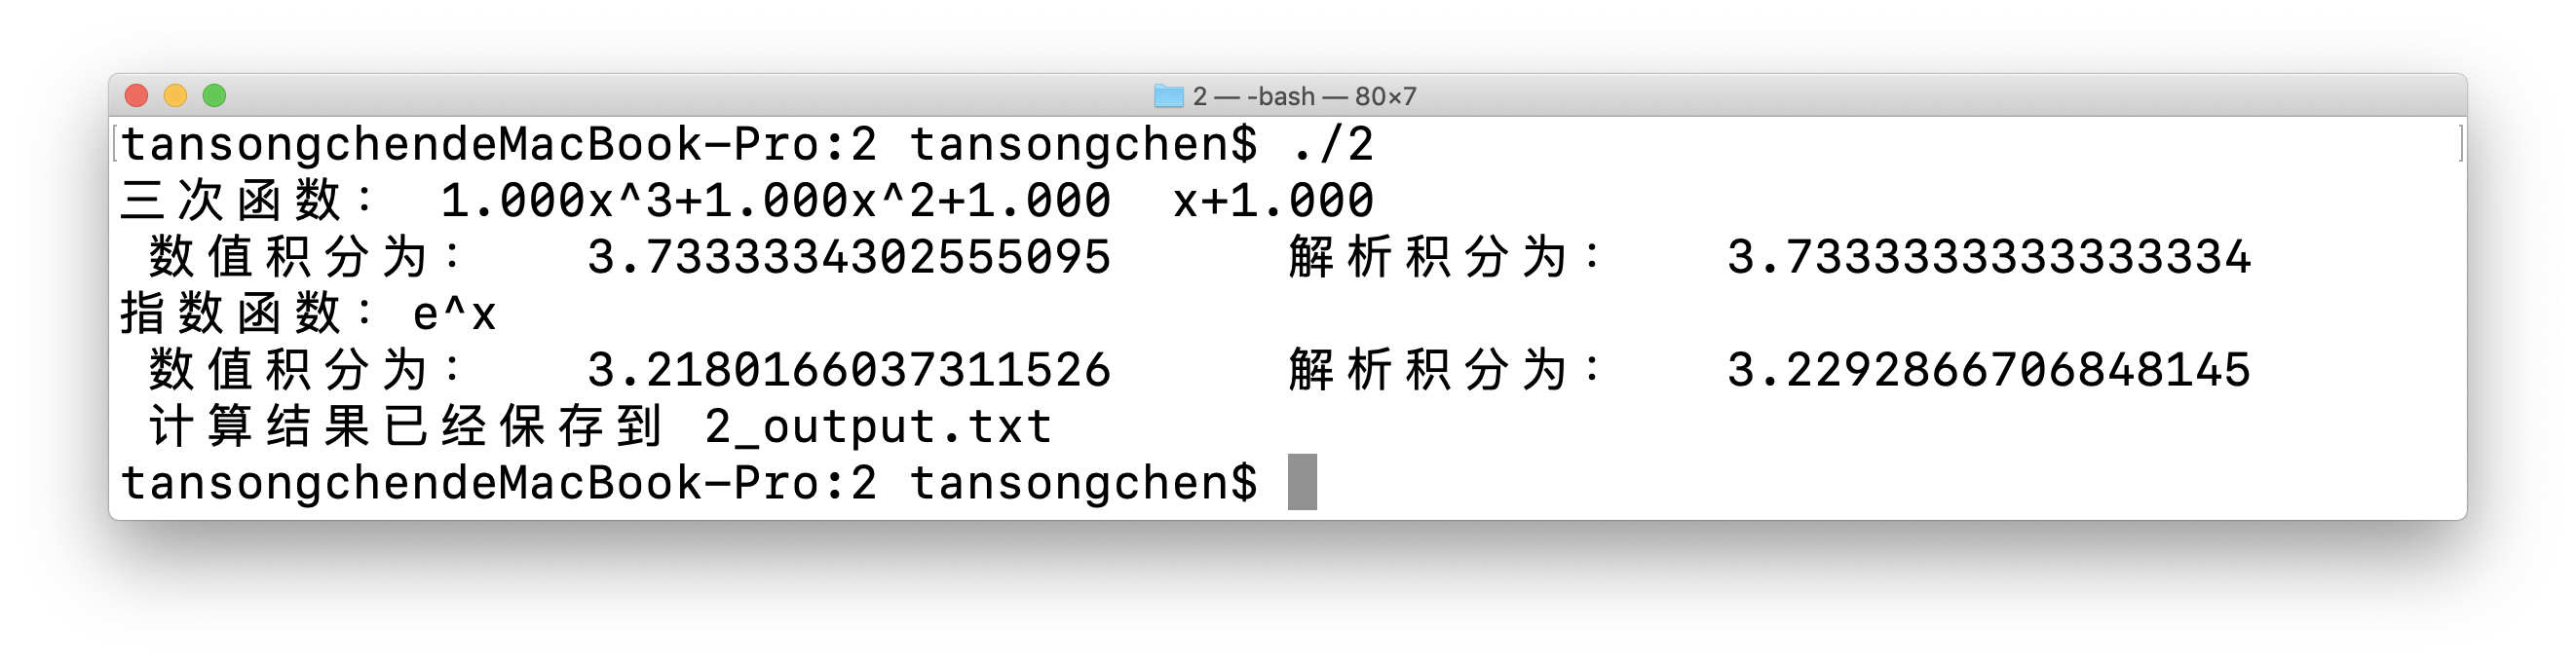
\includegraphics[scale = 0.3]{gauss.png}
\caption{Gauss 积分与解析积分的比较}
\end{figure}
可以看到,对三次函数两种积分方法给出的数值相等(微小的误差可能来源于平方根函数),而指数函数也只有 0.3\% 的误差。
\subsection{源代码}
\begin{lstlisting}
program project_2
	real*8, parameter :: a = 1, b = 1, c = 1, d = 1
	real*8, parameter :: x1 = sqrt(0.4), x2 = -sqrt(0.4)
	real*8, parameter :: C1 = 4.0/3.0, C2 = 4.0/3.0
	real*8 numerical_1, analytical_1, numerical_2, analytical_2

	open (unit = 11, file = '2_output.txt', status = 'replace')
	! 例 1: f = ax^3+bx^2+cx+d,应该得到精确解
	numerical_1 = C1*(a*x1**3+b*x1**2+c*x1+d) + &
	              C2*(a*x2**3+b*x2**2+c*x2+d)
	analytical_1 = 16*b/15+8*d/3
	write (*, '(A15,F6.3,A3,SPF6.3,A3,SPF6.3,A3,SPF6.3)') &
	'三次函数:', a, 'x^3', b, 'x^2', c, 'x', d
	write (*, *) &
	'数值积分为:', numerical_1, '解析积分为:', analytical_1
	! 例 2: f = e^x = 1+x+x^2/2+x^3/6...,前四项拟合精度尚可
	numerical_2 = C1*exp(x1) + C2*exp(x2)
	analytical_2 = 2*exp(1.0) - 6*exp(-1.0)
	write (*, '(A15,A3)') &
	'指数函数:', 'e^x'
	write (*, *) &
	'数值积分为:', numerical_2, '解析积分为:', analytical_2
	write (11, *) 'cubic_num', numerical_1, 'cubic_anal', analytical_1
	write (11, *) 'exp_num', numerical_2, 'exp_anal', analytical_2
	write (*, *) '计算结果已经保存到 2_output.txt'
end program
\end{lstlisting}
\newpage
\section{微分方程求解}
\subsection{问题描述}
考虑 A 和 B 两类原子核随时间的放射衰变问题,t 时刻其布居数为 $N_A(t),N_B(t)$,满足以下方程组:
\[
\frac{\f N_A(t)}{\f t}=-\frac{N_A}{\tau_A}
\]
\[
\frac{\f N_B(t)}{\f t}=-\frac{N_B}{\tau_B}+\frac{N_A}{\tau_A}
\]
其中,$\tau_A,\tau_B$ 为衰变时间常数。设初始时刻 $N_A(0)=N_B(0)=1$:
\begin{enumerate}
    \item 给出上述方程解析解;
    \item 数值求解上述微分方程组;
    \item 固定 $\tau_A$=1~s,讨论$\tau_B$=0.1~s, 1~s, 10~s 下的短期和长期衰变行为;
    \item 选取 $\tau_B$=10~s这一情况,讨论数值算法误差,展示时间步长 $\Delta t$ 为 0.05~s, 0.1~s, 0.2~s 时与解析结果的比较。
\end{enumerate}
\subsection{解答思路}
\subsubsection{解析解}
首先解出 A 类原子的一阶线性齐次方程:
\[
N_A(t)=\exp(-t/\tau_A)
\]
然后将其代入到 B 类原子的方程,变为一阶线性非齐次方程
\[
\frac{\f N_B(t)}{\f t}=-\frac{N_B}{\tau_B}+\frac{\exp(-t/\tau_A)}{\tau_A}
\]
由积分公式可以得到
\[
N_B(t)=\exp(-t/\tau_B)\left[C+\int \frac{\exp(-t/\tau_A)}{\tau_A} \exp(t/\tau_B) \f t\right]
\]
当 $\tau_A\ne\tau_B$ 时,积分得到
\[
N_B(t)=\frac{\tau_B}{\tau_A-\tau_B}\exp(-t/\tau_A)+\frac{\tau_A-2\tau_B}{\tau_A-\tau_B}\exp(-t/\tau_B)
\]
当 $\tau_A=\tau_B$ 时,对上式求极限得到
\[
N_B(t)=\exp(-t/\tau_A)(1+t/\tau_A)
\]
\subsubsection{数值解}
先求第一个方程的解。

根据数值积分中的梯形公式,我们有
\[
N_A^{(i+1)}=N_A^{(i)}+\int_{t_i}^{t_{i+1}}-\frac{N_A}{\tau_A}\f t\approx N_A^{(i)}-\frac{\Delta t}2\left[\frac{N_A^{(i)}}{\tau_A}+\frac{N_A^{(i+1)}}{\tau_A}\right]
\]
就能解出下一步的值相当于上一步的值乘以一个固定的因子
\[
N_A^{(i+1)}=N_A^{(i)}\times \frac{2\tau_A-\Delta t}{2\tau_A+\Delta t}
\]

解出关于 A 的方程后,再考虑 B 的方程,同理可得
\[
N_B^{(i+1)}=N_B^{(i)}+\int_{t_i}^{t_{i+1}}-\frac{N_B}{\tau_B}+\frac{N_A}{\tau_A}\f t\approx N_B^{(i)}+\frac{\Delta t}2\left[\frac{N_A^{(i)}}{\tau_A}+\frac{N_A^{(i+1)}}{\tau_A}-\frac{N_B^{(i)}}{\tau_B}-\frac{N_B^{(i+1)}}{\tau_B}\right]
\]
就能解出
\[
N_B^{(i+1)}=\frac{N_B^{(i)}+\frac{\Delta t}2\left[\frac{N_A^{(i)}}{\tau_A}+\frac{N_A^{(i+1)}}{\tau_A}-\frac{N_B^{(i)}}{\tau_B}\right]}{1+\frac{\Delta t}{2\tau_B}}
\]
写成与上类似的形式
\[
N_B^{(i+1)}=N_B^{(i)}\times\frac{2\tau_B-\Delta t}{2\tau_B+\Delta t}+\frac{\Delta t(N_A^{(i)}+N_A^{(i+1)})}{2\tau_B+\Delta t}\times\frac{\tau_B}{\tau_A}
\]
\subsection{算法描述}
\begin{lstlisting}
输入:时间步长 t,解析解公式,数值解公式
输出:na, nb(数值解的数据)
      na_, nb_(解析解的数据)

! 对 A
forall (i=0:N) na_(i) = function of i ! 解析表达式的值,下同
do i=0, N-1
    na(i+1) = function of na(i) ! 迭代公式
! 对 B
if (ta == tb) then
    forall (i=0:N) nb_(i) = function of i
else
    forall (i=0:N) nb_(i) = function of i

do i=0, N-1
    nb(i+1) = function of nb(i), na(i), na(i+1)
\end{lstlisting}
\subsection{计算结果与讨论}
\subsubsection{第一问}
\paragraph{条件} 固定 $\tau_A$=1~s,讨论$\tau_B$=0.1~s, 1~s, 10~s 下的短期和长期衰变行为。

本问与算法无关,可直接采用解析解进行作图处理。认为「短期」为 1 $\tau_B$,「长期」为 10 $\tau_B$。

\begin{figure}[h]
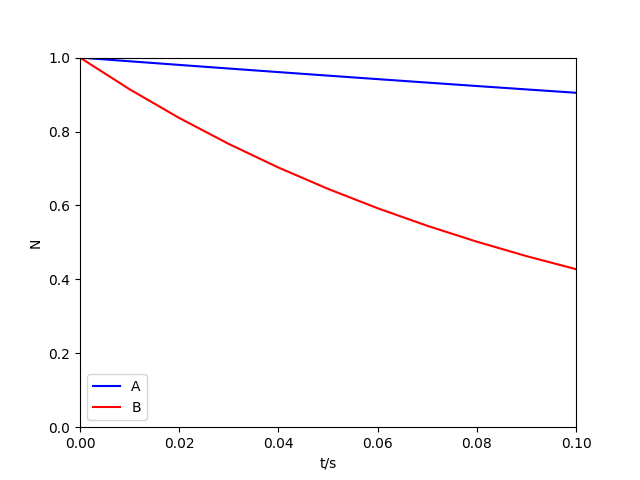
\includegraphics[scale = 0.4]{b01_s.png}
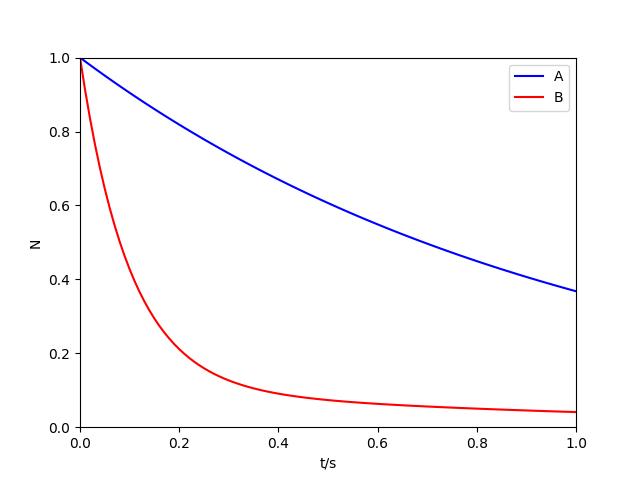
\includegraphics[scale = 0.4]{b01_l.png}
\caption{$\tau_B$ 为0.1~s 时的短期和长期衰变行为}
\end{figure}

$\tau_B$=0.1~s 时,短期,由于 B 的衰变速率显著快于 A,A 对 B 的影响不明显,几乎仍按指数衰减;但长期来看由于 A 的衰变速率慢,在后期仍有一定数量,此时 B 的数量已经很小,因此 A 衰变为 B 显著减慢了 B 衰变的速率,使其偏离指数衰减。

\begin{figure}[h]
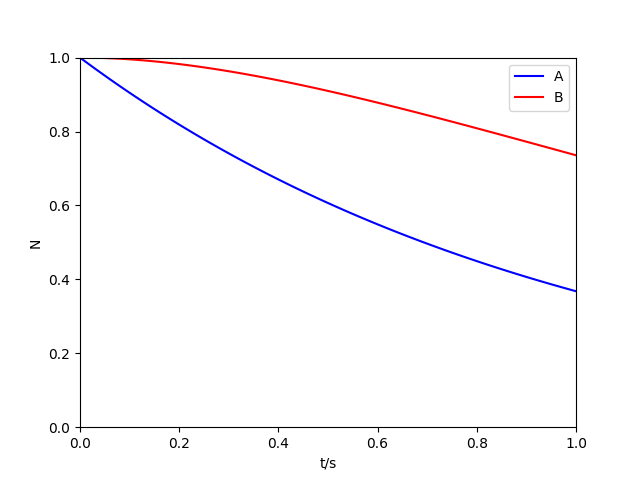
\includegraphics[scale = 0.4]{b1_s.png}
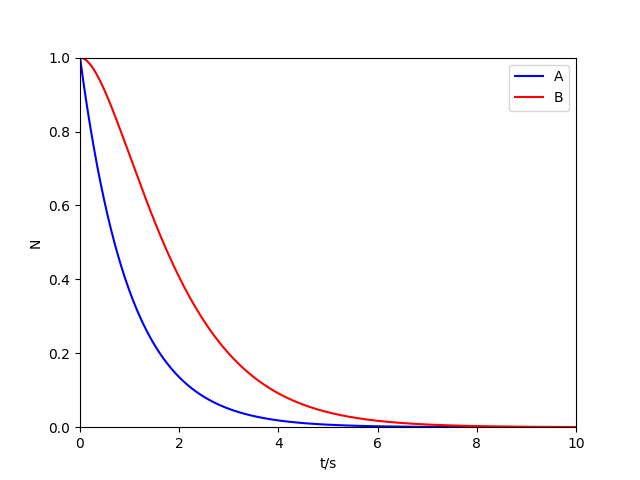
\includegraphics[scale = 0.4]{b1_l.png}
\caption{$\tau_B$ 为1~s 时的短期和长期衰变行为}
\end{figure}

$\tau_B$=1~s 时,短期,由于 B 的指数衰减叠加上了线性增长的因子,下降速率很慢且为凸函数;长期,随着 A 的数量减小这一作用逐渐降低,按正常指数衰减趋于 0。

\begin{figure}[h]
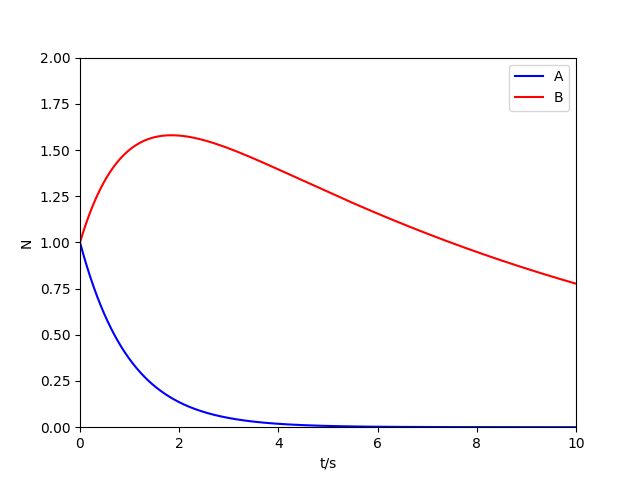
\includegraphics[scale = 0.4]{b10_s.png}
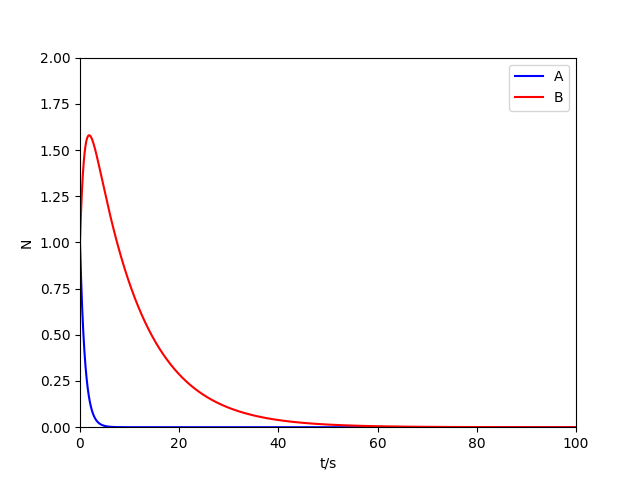
\includegraphics[scale = 0.4]{b10_l.png}
\caption{$\tau_B$ 为10~s 时的短期和长期衰变行为}
\end{figure}

$\tau_B$=10~s 时,短期,A 衰变为 B 使 B 的数量不降反增;长期,随着 A 的数量减小这一作用逐渐降低,先转折然后按正常指数衰减趋于 0。

\subsubsection{第二问}
\paragraph{条件} 选取 $\tau_B$=10~s这一情况,讨论数值算法误差,展示时间步长 $\Delta t$ 为 0.05~s, 0.1~s, 0.2~s 时与解析结果的比较。

数值算法的误差本质上来源于对积分的近似处理。根据数值积分的误差估计公式,梯形法得到的积分应该使得误差为 $O((\Delta t)^2)$,而如果仅采用端点值,误差为 $O(\Delta t)$。

如果采用更高阶的积分公式,误差将得到进一步降低,但此时需要求解非线性方程,考虑到计算量,在梯形公式中取更小的步长是更经济的做法。根据图 5,我们可以选择计算区间为 4 $\tau_B$。我们将可以在下面的数值模拟中看到,在取时间步长为 0.2~s 时, 4 $\tau_B$ 内,数值结果与解析结果没有明显差别(实线为解析解,虚线为数值解),而取更小的时间步长时效果将更好。

\begin{figure}[h]
\centering
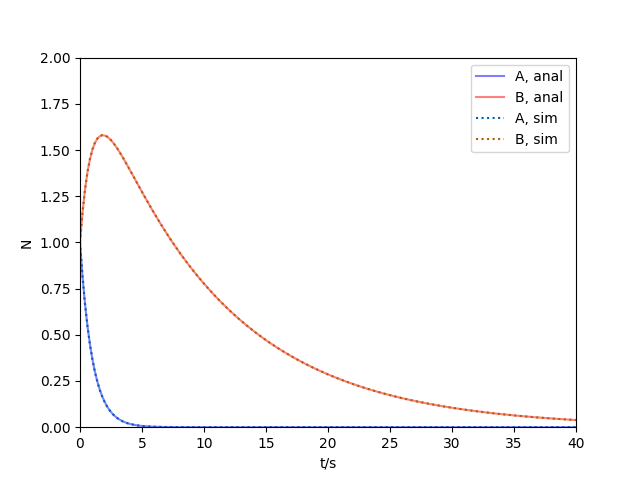
\includegraphics[scale = 0.5]{sim.png}
\caption{$\Delta t$ 为 0.2~s 时的模拟结果}
\end{figure}

进行定量的误差分析,在 0 到 4 $\tau_B$ 范围内,数值模拟产生的最大的绝对误差列于下图中。

\begin{figure}[h]
\centering
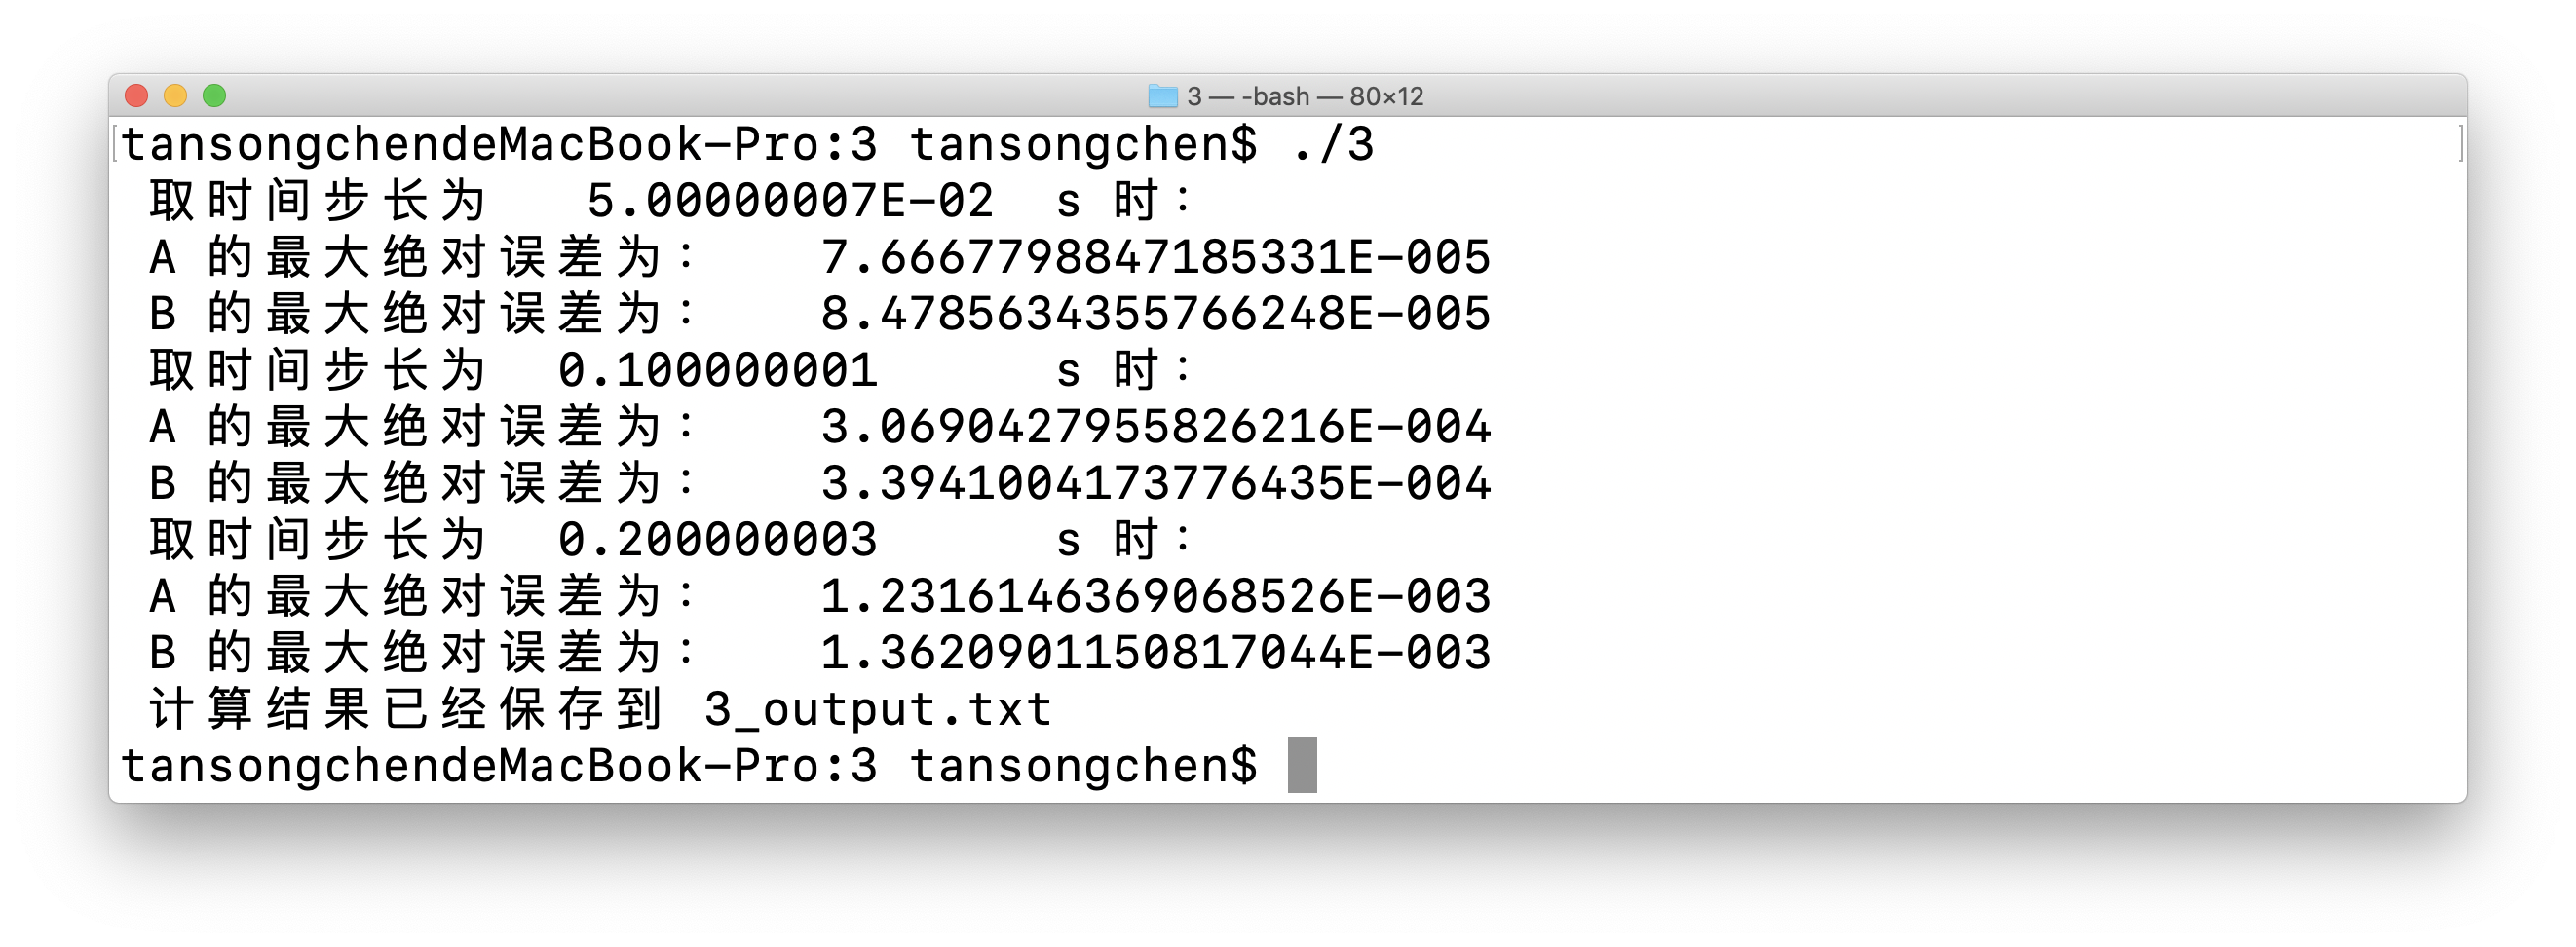
\includegraphics[scale = 0.3]{error.png}
\caption{不同 $\Delta t$ 时的模拟误差}
\end{figure}

可见当步长减小为原来的 1/2 时,误差减小为原来的 1/4,符合我们之前分析的误差为 $O((\Delta t)^2)$ 的结论。
\subsection{源代码}
\begin{lstlisting}
program project3
	real*8, parameter :: ta = 1, tb = 10, dt(3) = (/0.05, 0.1, 0.2/)
	real*8, allocatable :: na(:), nb(:), na_(:), nb_(:)
	integer i, j, N

	open (11, file = '3_output.txt')
	do j=1, 3
		t = dt(j)
		N = nint(4*tb/t)
		allocate(na(N), nb(N), na_(N), nb_(N))
		na(0)=1
		nb(0)=1
		forall (i=0:N) na_(i) = exp(-i*t/ta)
		do i=0, N-1
			na(i+1) = na(i)*(2*ta-t)/(2*ta+t)
		end do
		if (ta == tb) then
			forall (i=0:N) nb_(i) = exp(-i*t/ta)*(1+i*t/ta)
		else
			forall (i=0:N) nb_(i) = (exp(-i*t/ta)*tb+&
			exp(-i*t/tb)*(ta-2*tb))/(ta-tb)
		end if
		do i=0, N-1
			nb(i+1) = nb(i)*(2*tb-t)/(2*tb+t)+&
			tb/ta*t/(2*tb+t)*(na(i+1)+na(i))
		end do
		write (*, *) '取时间步长为', t, ' s 时:'
		write (*, *) 'A 的最大绝对误差为:', maxval(abs(na-na_))
		write (*, *) 'B 的最大绝对误差为:', maxval(abs(nb-nb_))
		write (11, *) '时间步长为', t, '时,A 的数值解:'
		write (11, *) na
		write (11, *) '时间步长为', t, '时,A 的解析解:'
		write (11, *) na_
		write (11, *) '时间步长为', t, '时,B 的数值解:'
		write (11, *) nb
		write (11, *) '时间步长为', t, '时,B 的解析解:'
		write (11, *) nb_
		deallocate(na, nb, na_, nb_)
	end do
	write (*, *) '计算结果已经保存到 3_output.txt'
end program
\end{lstlisting}
\newpage
\section{三次样条插值}
\subsection{问题描述}
已知离散数据点如下表,试用三次样条插值法获得 $x$ 每间隔 $0.1$ m 时 $y$ 的取值。

\begin{table}[h]
\centering
\caption{插值的原始数据}
\begin{tabular}{cc}
\toprule
$x$/m & $y$/m \\ \midrule
0     & 0.0   \\
3     & 1.2   \\
5     & 1.7   \\
7     & 2.0   \\
9     & 2.1   \\
11    & 2.0   \\
12    & 1.8   \\
13    & 1.2   \\
14    & 1.0   \\
15    & 1.6   \\ \bottomrule
\end{tabular}
\end{table}
\subsection{解答思路}
根据三次样条插值法,加入自然边界条件(边界处给出二阶导数的值且为0)后,得到如下的三弯矩方程,其中系数矩阵为对称正定三对角阵。

\[
\left[ \begin{array}{ccccc}
{2} & {\lambda_{1}} & & & \\
{\mu_{2}} & {2} & {\lambda_{2}} & { } & { } \\
{ } & {\ddots} & {\ddots} & {\ddots} & { } \\
{ } & { } & {\mu_{n-2}} & {2} & {\lambda_{n-2}} \\
{ } & { } & { } & {\mu_{n-1}} & {2}
\end{array}\right]
\left[ \begin{array}{c}{M_{1}} \\ {M_{2}} \\ {\vdots} \\ {M_{n-2}} \\ {M_{n-1}}\end{array}\right]
=
\left[ \begin{array}{c}{d_{1}} \\ {d_{2}} \\ {\vdots} \\ {d_{n-2}} \\ {d_{n-1}}\end{array}\right]
\]

利用追赶法解上述方程,得各插值点的二阶导数,按下式得到各段的三次函数。

\[
S(x)=\frac{\left(x_{j+1}-x\right)^{3}}{6 h_{j}} M_{j}+\frac{\left(x-x_{j}\right)^{3}}{6 h_{j}} M_{j+1}+c_{1} x+c_{2}
\]
\[
c_{1}=\frac{y_{j+1}-y_{j}}{h_{j}}-\frac{1}{6} h_{j}\left(M_{j+1}-M_{j}\right)
\]
\[
c_{2}=\frac{y_{j} x_{j+1}-y_{j+1} x_{j}}{h_{j}}-\frac{1}{6} h_{j}\left(x_{j+1} M_{j}-x_{j} M_{j+1}\right)
\]

在本题中,由于 $x$ 均为整数,可以简化最后求值的过程:对原始 $x$ 数据点进行遍历,在每个点向后计算 $(x_{i+1}-x_i)\times 10$ 个点即得到所有 151 个点 $y$ 的表达式,避免判断某一个特定的 $x$ 落在哪一个三次样条函数的区间内。

\subsection{算法描述}
\begin{lstlisting}
输入:x(0:9), y(0:9)
输出:y_new(0:150)

! 根据定义计算方程系数
forall (i=0:n-1) h(i) = x(i+1)-x(i)
forall (i=1:n-1) d(i) = 6F[x(i-1),x(i),x(i+1)]
forall (i=2:n-1) mu(i) = h(i-1)/(h(i-1)+h(i))
forall (i=1:n-2) lambda(i) = h(i)/(h(i-1)+h(i))

! 追赶法解方程,首先进行分解
do i=2, n-1
    q = mu(i)/b(i-1)
    b(i) = b(i)-q*lambda(i-1)
    d(i) = d(i)-q*d(i-1)

! 回代求解
m(n-1) = d(n-1)/b(n-1)
do i=n-2, 1, -1
    m(i) = (d(i)-lambda(i)*m(i+1))/b(i)

! 根据三次样条函数方程求 y 的值
do i=0, n-1
    c1 = ...
    c2 = ...
    do j=0, 10*h(i)
        xn = x(i)+j*0.1
        y_new(10*xn) = ...

write y_new
\end{lstlisting}
\subsection{计算结果与讨论}
三次样条插值得到的曲线能较好地平滑拟合这些数据点。
\begin{figure}[h]
\centering
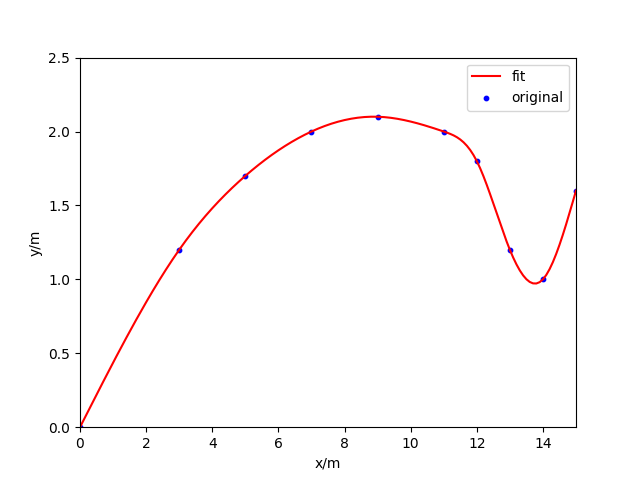
\includegraphics[scale = 0.6]{spline.png}
\caption{三次样条插值得到的曲线与原始数据点}
\end{figure}
\subsection{源代码}
\begin{lstlisting}
program project4
	integer, parameter :: n = 9
	real*8, parameter :: x(0:n) = (/0, 3, 5, 7, 9, &
		                          11, 12, 13, 14, 15/)
	real*8, parameter :: y(0:n) = (/0.0, 1.2, 1.7, 2.0, &
		                          2.1, 2.0, 1.8, 1.2, 1.0, 1.6/)
	real*8 :: x_new(0:nint(x(n)*10)) = &
	(/(i*0.1, i = 0, nint(x(n)*10))/)
	real*8 :: y_new(0:nint(x(n)*10)) = 0.0
	real*8 :: h(0:n-1) = 0.0, d(1:n-1) = 0.0, m(0:n) = 0.0
	real*8 :: lambda(1:n-2) = 0.0, mu(2:n-1) = 0.0, b(1:n-1) = 2
	real*8 :: c1, c2, q, xn

	! 根据定义计算方程系数
	forall (i=0:n-1) h(i) = x(i+1)-x(i)
	forall (i=1:n-1) d(i) = ((y(i+1)-y(i))/h(i)-(y(i)-y(i-1)) & 
	/h(i-1))*6/(h(i-1)+h(i))
	forall (i=2:n-1) mu(i) = h(i-1)/(h(i-1)+h(i))
	forall (i=1:n-2) lambda(i) = h(i)/(h(i-1)+h(i))

	! 追赶法解方程,首先进行分解
	do i=2, n-1
		q = mu(i)/b(i-1)
		b(i) = b(i)-q*lambda(i-1)
		d(i) = d(i)-q*d(i-1)
	end do
	! 回代求解
	m(n-1) = d(n-1)/b(n-1)
	do i=n-2, 1, -1
		m(i) = (d(i)-lambda(i)*m(i+1))/b(i)
	end do

	! 根据三次样条函数方程求 y 的值
	do i=0, n-1
		c1 = (y(i+1)-y(i))/h(i)-h(i)*(m(i+1)-m(i))/6
		c2 = (y(i)*x(i+1)-y(i+1)*x(i))/h(i)- & 
		     h(i)*(x(i+1)*m(i)-x(i)*m(i+1))/6
		do j=0, nint(h(i))*10
			xn = x(i)+j*0.1
			y_new(nint(10*xn)) = (x(i+1)-xn)**3*m(i)/6/h(i)+ &
			                     (xn-x(i))**3*m(i+1)/6/h(i)+ &
			                     c1*xn+c2
		end do
	end do
	open (11, file = '4_output.txt')
	write (11, *) y_new
	write (*, *) '计算结果已经保存到 4_output.txt'
end program
\end{lstlisting}
\newpage
\section{对称正定带状矩阵系数方程组的直接求解}
\subsection{问题描述}
用对称正定带状矩阵系数方程组的一般解法解 $n$ 阶方程,$n = 100, 10000$。

系数矩阵 $\mathbf A$ 满足 $m=2$,非零元素 $a_{11}=a_{nn}=5,a_{ii}=6(2\le i\le n-1)$,$a_{i,i-1}=4(2\le i\le n)$,$a_{i,i-2}=1(3\le i\le n)$。

右端向量 $\mathbf b$ 为 $(60, 120, ..., 120, 60)^T$。

\[
\left[ \begin{array}{llllllll}
{5} & {4} & {1} & {0} & {0} & {\cdots} & {0} & {0} \\ 
{4} & {6} & {4} & {1} & {0} & {\cdots} & {0} & {0} \\ 
{1} & {4} & {6} & {4} & {1} & {\cdots} & {0} & {0} \\ 
{0} & {1} & {4} & {6} & {4} & {\cdots} & {0} & {0} \\ 
{0} & {0} & {1} & {4} & {6} & {\cdots} & {0} & {0} \\ 
{\vdots} & {\vdots} & {\vdots} & {\vdots} & {\vdots} & { } & {\vdots} & {\vdots} \\ 
{0} & {0} & {0} & {0} & {0} & {\cdots} & {6} & {4} \\ 
{0} & {0} & {0} & {0} & {0} & {\cdots} & {4} & {5}\end{array}\right] 
\left[ \begin{array}{c}{x_{1}} \\ {x_{2}} \\ {x_{3}} \\ {x_{3}} \\ {\vdots} \\ {x_{n-2}} \\ {x_{n-1}} \\ {x_{n}}\end{array}\right]=\left[ \begin{array}{c}{60} \\ {120} \\ {120} \\ {120} \\ {120} \\ {\vdots} \\ {120} \\ {00}\end{array}\right]
\]
\subsection{解答思路}
降低空间复杂度要求我们将系数矩阵和分解产生的下三角矩阵以 $n\times 3$ 矩阵存储。在 $n\times n$ 矩阵中表示的求解公式课件已经给出:(将分解后的右端向量记为 $\mathbf e$)

\[
l_{ij} = a_{ij} - \sum_{k=r}^{j-1}l_{ik}l_{jk}/l_{kk}
\]

\[
e_i=b_i-\sum_{j=r}^{i-1}l_{ij}e_j/l_{jj}
\]

\[
x_i=\left(e_i-\sum_{j=i+1}^tl_{ji}x_j\right)/l_{ii}
\]

上三式中

\[
r = 
\begin{cases}
1, & i \le 3\\
i-2, & i > 3
\end{cases}
, \qquad t = 
\begin{cases}
n, & i > n-3\\
i+2, & i\le n-3
\end{cases}
\]

为了去掉这些条件判断,增加定义冗余元素 $l_{00}=1, l_{1-1}=l_{10}=l_{20}=0, b_{n+1}=b_{n+2}=0$,就可以将 $r$ 统一为 $i-2$,$t$ 统一为 $i+2$。

下面进行推导将其变换到 $n\times 3$ 矩阵中:
\subsubsection{系数矩阵分解}

记用 $n\times 3$ 矩阵表示的系数矩阵和下三角矩阵分别为 $\mathbf C,\mathbf M$。则有:

\begin{multline}
m_{ij}=l_{i,j+i-3} = a_{i,j+i-3} - \sum_{k=i-2}^{j+i-4}l_{ik}l_{j+i-3,k}/l_{kk}\\
=c_{ij}-\sum_{k=i-2}^{j+i-4}m_{i,k+i-3}m_{j+i-3,k-j-i+6}/m_{k3}\\
=c_{ij}-\sum_{p=1}^{j-1}m_{ip}m_{j+i-3,p-j+3}/m_{p+i-3,3}\\
\end{multline}

由于 $m_{ij}$ 的 $j$ 只能取 $1,2,3$ 这三种情况,故将这三种情况代入上式,分别列出:

\[
m_{i1} = c_{i1}
\]
\[
m_{i2} = c_{i2} - m_{i1}m_{i-1,2}/m_{i-2,3}
\]
\[
m_{i3} = c_{i3} - m_{i1}m_{i1}/m_{i-2,3} - m_{i2}m_{i2}/m_{i-1,3}
\]

\subsubsection{右端向量分解}

\begin{multline}
e_i=b_i-\sum_{j=i-2}^{i-1}l_{ij}e_j/l_{jj}\\
=b_i-\sum_{j=i-2}^{i-1}m_{i,j-i+3}e_j/m_{j3}\\
=b_i-m_{i1}e_{i-2}/l_{i-2,3}-m_{i2}e_{i-1}/m_{i-1,3}\\
\end{multline}

\subsubsection{回代求解}

\begin{multline}
x_i=\left(e_i-\sum_{j=i+1}^{i+2}l_{ji}x_j\right)/l_{ii}\\
=\left(e_i-\sum_{j=i+1}^{i+2}m_{j,i-j+3}x_j\right)/m_{i3}\\
=\left(e_i-m_{i+1,2}x_{i+1}-m_{i+2,1}x_{i+2}\right)/m_{i3}\\
\end{multline}

在实际编写程序时,用原地工作的方式,三个向量存储矩阵 $\mathbf C$,一个向量存储右端向量 $\mathbf b$,按 5.2.1 中的公式 $\mathbf M$ 覆盖 $\mathbf C$,按 5.2.2 中的公式 $\mathbf e$ 覆盖 $\mathbf b$,按 5.2.3 中的公式 $\mathbf x$ 覆盖 $\mathbf e$。
\subsection{算法描述}
\begin{lstlisting}
输入:n, a1, a2, a3, b
输出:b(也就是 x)

! 分解为下三角矩阵 L
do i = 2, n
    a2(i) = ...
    a3(i) = ...

! 对右端向量也作分解
do i = 2, n
    b(i) = ...

! 回代解方程
do i = n, 1, -1
    b(i) = ...

write b
\end{lstlisting}
\subsection{计算结果与讨论}
由于数据量较大,不展示输出结果,而是作 $x_i\sim i$ 图以定性展示解的行为($n$ = 10000 时解的纵坐标刻度为 $10^7$)。


\begin{figure}[ht]
\centering
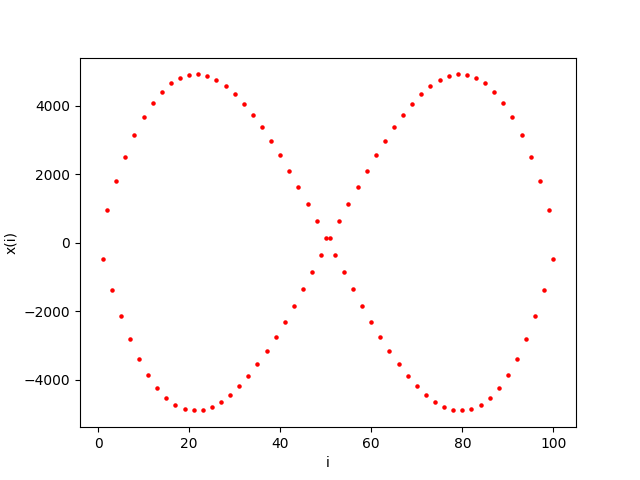
\includegraphics[scale = 0.5]{eqn100.png}
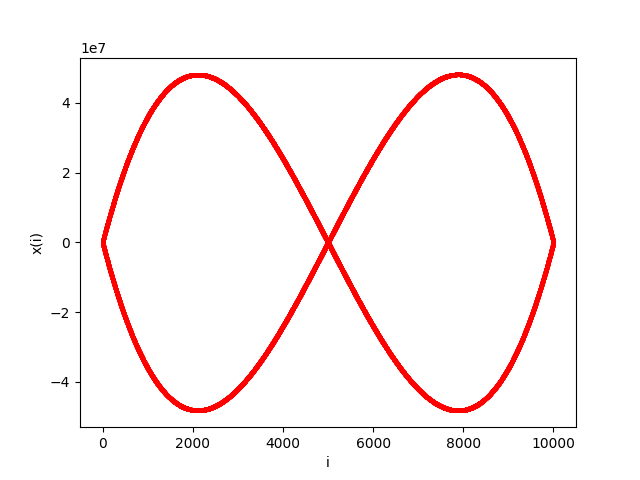
\includegraphics[scale = 0.5]{eqn10000.png}
\caption{$n$ = 100(左)和 10000(右)时解随指标的变化规律}
\end{figure}

\subsection{源代码}
\begin{lstlisting}
program project5
	integer, parameter :: ns(2) = (/100, 10000/)
	real*8, allocatable :: a1(:), a2(:), a3(:), b(:)
	integer i, j

	open (11, file = '5_output.txt')
	do j = 1, 2
		n = ns(j)
		allocate(a1(0:n+2),a2(0:n+2),a3(0:n+2),b(0:n+2))
		! 向量赋初值时,多放几个冗余的元素
		! 便于循环时不用作额外的判断
		a1(0:n+2) = (/1.0, 0.0, 0.0, (1.0, i=3, n), 0.0, 0.0/)
		a2(0:n+2) = (/1.0, 0.0, (4.0, j=2, n), 0.0, 0.0/)
		a3(0:n+2) = (/1.0, 5.0, (6.0, k=2, n-1), 5.0, 0.0, 0.0/)
		b(0:n+2) = (/0.0, 60.0, (120.0, i=2, n-1), 60.0, 0.0, 0.0/)
		! 分解为下三角矩阵 L
		do i = 2, n
			a2(i) = a2(i) - a1(i)*a2(i-1)/a3(i-2)
			a3(i) = a3(i) - a1(i)*a1(i)/a3(i-2) - &
			a2(i)*a2(i)/a3(i-1)
		end do
		! 对右端向量也作分解
		do i = 2, n
			b(i) = b(i) - a1(i)*b(i-2)/a3(i-2) - &
			a2(i)*b(i-1)/a3(i-1)
		end do
		! 回代解方程
		do i = n, 1, -1
			b(i) = (b(i) - a2(i+1)*b(i+1) - &
			a1(i+2)*b(i+2))/a3(i)
		end do
		write (11, *) 'n 取', n, '时的解:'
		write (11, *) b(1:n)
		write (*, *) 'n 取', n, &
		'时的解计算完成,解保存到 5_output.txt'
		deallocate(a1, a2, a3, b)
	end do
end program
\end{lstlisting}
\newpage
\section{稀疏矩阵系数方程组的共轭梯度法迭代求解}
\subsection{问题描述}
用对称正定矩阵的共轭梯度法解 $n$ 阶方程,$n = 100, 10000$。

系数矩阵 $\mathbf A$ 的非零元素 $a_{ii}=3(1\le i\le n)$,$a_{i,i+1}=a_{i+1,i}=-1(1\le i\le n-1)$,不在上述三对角线上但在副对角线上的元素 $a_{i,n+1-i}=1(3\le i\le n)$。

右端向量 $\mathbf b$ 为 $(2.5, 1.5, ..., 1.0, 1.0, 1.5, ..., 2.5)^T$。

\[
\left[\begin{array}{cccccc}
3 & -1 & 0 & \cdots & 0 & 1/2 \\
-1 & 3 & -1 & \cdots & 1/2 & 0 \\
\vdots & \vdots & \vdots & \vdots & \vdots & \vdots \\
0 & 0 & 0 & \cdots & 0 & 0 \\
0 & 0 & 0 & \cdots & 0 & 0 \\
\vdots & \vdots & \vdots & \vdots & \vdots & \vdots \\
0 & 1/2 & 0 & \cdots & 3 & -1 \\
1/2 & 0 & 0 & \cdots & -1 & 3\\
\end{array}\right]
\left[ \begin{array}{c}{x_{1}} \\ {x_{2}} \\ {\vdots} \\ x_{n/2} \\ x_{n/2+1}\\ {\vdots}  \\ {x_{n-1}} \\ {x_{n}}\end{array}\right]=\left[ \begin{array}{c}{2.5} \\ {1.5} \\ {\vdots} \\ {1.0} \\ {1.0} \\ {\vdots} \\ {1.5} \\ {2.5}\end{array}\right]
\]

\subsection{解答思路}
容易看出该方程的精确解即为 $(1.0, ..., 1.0)^T$。

观察算法,发现循环中共需要算 4 次模方(1 次$\tilde{\mathbf r}^T\tilde{\mathbf r}$,3 次 $\mathbf r^T\mathbf r$),2 次矩阵乘法($\mathbf A\mathbf p$),1 次内积($\mathbf p^T\mathbf A\mathbf p$)。为了节省计算量,将残差向量的模方计算出来之后用变量 \verb|r2, rlast2| 储存起来,可以避免重复计算。同时,为了节省存储空间,不存储矩阵 $\mathbf A$,而是将它与向量 $\mathbf p$ 的乘法表述为某种函数的形式。推导如下:

首先将 $\mathbf A$ 拆分,对角线上元素归为数量矩阵,对角线上下的元素归为不完全移位矩阵,副对角线上元素归为一个副对角矩阵减去两个基本矩阵。

\[
\mathbf A= 3\mathbf I - \mathbf A_1 - \mathbf A_2 + \frac12\left[\mathbf A_3 - \mathbf E_{n/2,n/2+1} - \mathbf E_{n/2+1,n/2}\right]
\]

\[
\mathbf A_1 = 
\left[\begin{array}{cccccc}
0 & 1 & 0 & \cdots & 0 & 0 \\
0 & 0 & 1 & \cdots & 0 & 0 \\
0 & 0 & 0 & \cdots & 0 & 0 \\
\vdots & \vdots & \vdots & \vdots & \vdots & \vdots \\
0 & 0 & 0 & \cdots & 0 & 1 \\
0 & 0 & 0 & \cdots & 0 & 0\\
\end{array}\right]
\]
\[
\mathbf A_2 = 
\left[\begin{array}{cccccc}
0 & 0 & 0 & \cdots & 0 & 0 \\
1 & 0 & 0 & \cdots & 0 & 0 \\
0 & 1 & 0 & \cdots & 0 & 0 \\
\vdots & \vdots & \vdots & \vdots & \vdots & \vdots \\
0 & 0 & 0 & \cdots & 0 & 0 \\
0 & 0 & 0 & \cdots & 1 & 0\\
\end{array}\right]
\]
\[
\mathbf A_3 = 
\left[\begin{array}{cccccc}
0 & 0 & 0 & \cdots & 0 & 1 \\
0 & 0 & 0 & \cdots & 1 & 0 \\
0 & 0 & 0 & \cdots & 0 & 0 \\
\vdots & \vdots & \vdots & \vdots & \vdots & \vdots \\
0 & 1 & 0 & \cdots & 0 & 0 \\
1 & 0 & 0 & \cdots & 0 & 0\\
\end{array}\right]
\]

由矩阵乘法的定义推知,$\mathbf I\mathbf p=\mathbf p$,$\mathbf A_1\mathbf p=(p_2, p_3, ..., p_n, 0)^T$,$\mathbf A_2\mathbf p=(0, p_1, ..., p_{n-2}, p_{n-1})^T$,$\mathbf A_3\mathbf p=(p_n, p_{n-1}, ..., p_1)^T$。

在实现向量错位相加时,可以如同上题一样定义冗余元素 $p_0=0, p_{n+1}=0$,以减少判断。

\subsection{算法描述}
\begin{lstlisting}
输入:A(隐含在计算中),b,x
输出:x,times(迭代次数)

r = b - A * x
p = r
r2 = (r,r)
do while (r2 > 1D-12)
    times = times + 1
    Ap = A * p
    alpha = r2/(p,Ap)
    x = x + alpha * p
    r = r - alpha * Ap
    rlast2 = r2
    r2 = (r,r)
    beta = r2/rlast2
    p = r + beta * p
write x, times
\end{lstlisting}
\subsection{计算结果与讨论}
统计 $n=100, 10000$ 时所需要的迭代次数,发现均为 15 次,这说明共轭梯度法具有很高的效率。

\begin{figure}[h]
\centering
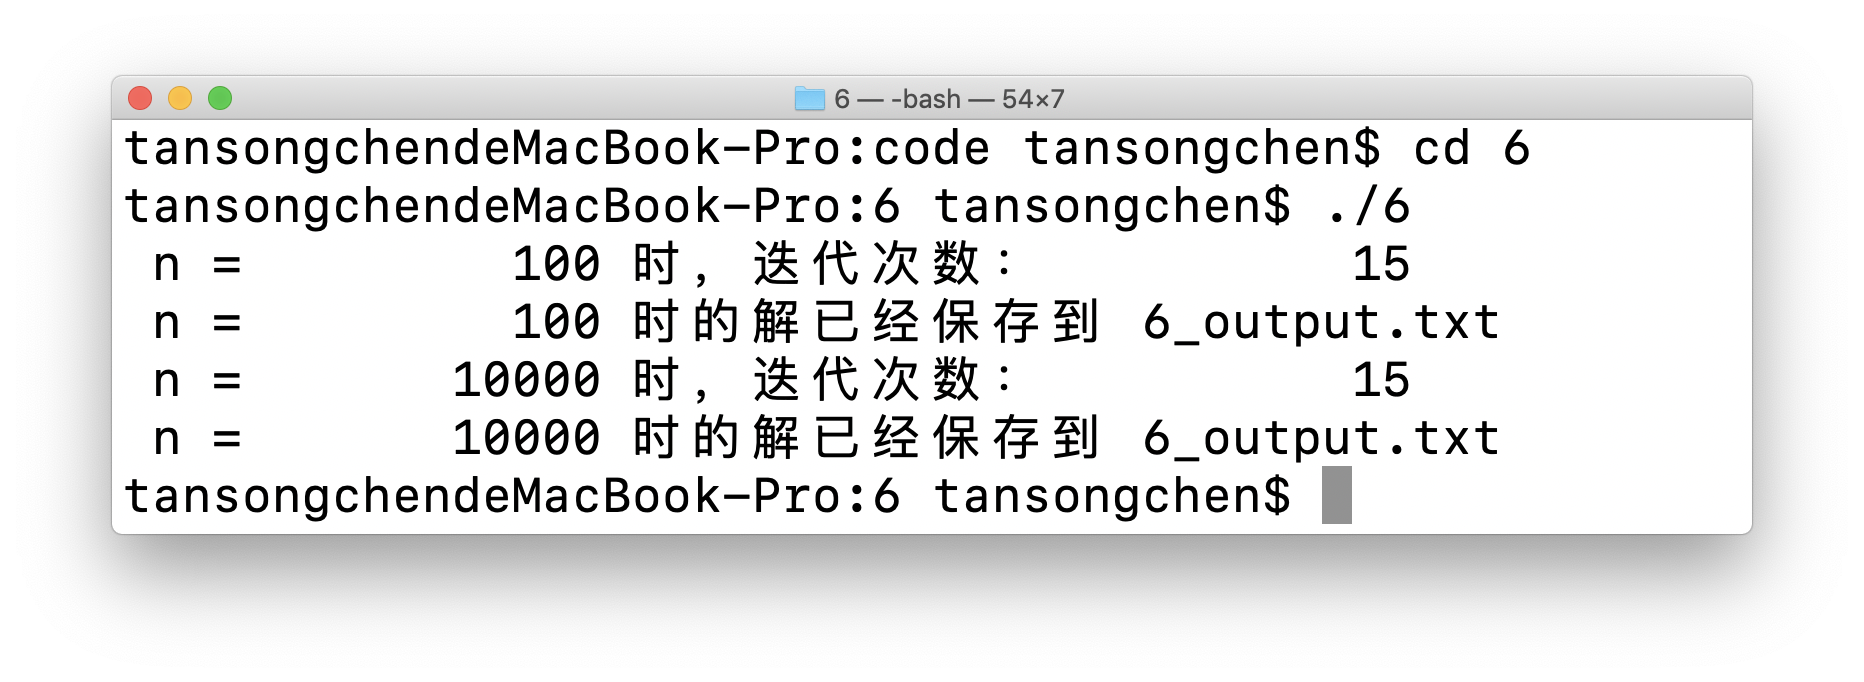
\includegraphics[scale = 0.4]{conj.png}
\caption{共轭梯度法解方程}
\end{figure}

进行另外的尝试,更换其中的判停标准为 $\mathbf r^T\mathbf r<10^{-20}$,发现迭代次数变为 23 次。这说明每迭代一次,解的有效数字约增加半位。

本解法中采取助教提供的作业提示中计算残差向量范数 $||\mathbf r||<10^{-6}$,也即 $\mathbf r^T\mathbf r<10^{-12}$ 作为判停标准(因为模方已经在计算过程中用到,利用它判断无需额外计算)。原题目中要求判停标准为相邻两次迭代解之差的范数 $<10^{-6}$,在本算法中只要在更新完解之后计算一次 $\alpha^2 \mathbf p^T\mathbf p$ 即可。
\subsection{源代码}
\begin{lstlisting}
program project6
	integer, parameter :: ns(2) = (/100, 10000/)
	real*8, allocatable :: b(:), r(:), x(:), p(:), Ap(:), Ax(:)
	real*8 :: alpha, beta, r2, rlast2
	integer :: times = 0, i

	open (11, file = '6_output.txt')
	do i = 1, 2
		times = 0
		n = ns(i)
		! 根据参数申请内存,并给初值
	    ! 增加冗余元素,方便计算乘积
		allocate(b(0:n+1), r(0:n+1), x(0:n+1), p(0:n+1))
		allocate(Ax(0:n+1), Ap(0:n+1))
		x = 0
		b(0:n+1) = (/0.0, 2.5, (1.5, I=2, n/2-1), 1.0, &
		           1.0, (1.5, I=n/2+2, n-1), 2.5, 0.0/)
		! 计算初始残差
		Ax(1:n) = 3.0 * x(1:n) - x(2:n+1) - x(0:n-1) + &
			          0.5 * x(n:1:-1)
		Ax(n/2:n/2+1) = Ax(n/2:n/2+1) - 0.5 * x(n/2+1:n/2:-1)
		r = b - Ax
		p = r
		r2 = dot_product(r,r)
		do while (r2 > 1D-12)
			times = times + 1
			! 计算矩阵乘法
			Ap(1:n) = 3.0 * p(1:n) - p(2:n+1) - p(0:n-1) + &
			          0.5 * p(n:1:-1)
			Ap(n/2:n/2+1) = Ap(n/2:n/2+1) - &
			0.5 * p(n/2+1:n/2:-1)
			! 更新解
			alpha = r2/dot_product(p,Ap)
			x = x + alpha * p
			! 更新残差向量
			r = r - alpha * Ap
			rlast2 = r2
			! 计算新的残差向量模方
			r2 = dot_product(r,r)
			! 更新方向
			beta = r2/rlast2
			p = r + beta * p
		end do
		write(*, *) 'n =', n, '时,迭代次数:', times
		write(11, *) 'n =', n, '时,解为:'
		write(11, *) x(1:n)
		write(*, *) 'n =', n, '时的解已经保存到 6_output.txt'
		deallocate(b, r, x, p, Ax, Ap)
	end do
end program
\end{lstlisting}
\newpage
\section{Laguerre 多项式的递推求值}
\paragraph{注} 大作业中的第七题因体量较大,本文中将第 1 问归于 Section 7,第 2、3 问归于 Section 8,第 4 问归于 Section 9 分别撰写。
\subsection{问题描述}
求广义 Laguerre 多项式 $L_n^\alpha(x)$ 在如下情况时的值:$n=3, 10, 30; \alpha=2, 20, 40;x=0.001, 1, 100$。
\subsection{解答思路}
从作业中给出的两个递推关系出发,我们可以找到一个更加简洁的递推关系:
\[
L_{n+1}^\alpha(x)=\frac{(2n+1-\alpha-x)L_{n}^\alpha(x)-(n+\alpha)L_{n-1}^\alpha(x)}{n+1}
\]

这个公式的好处是 $\alpha$ 不会改变,因此可以直接用线性递推公式求出:$L_0^\alpha,L_1^\alpha\Rightarrow L_2^\alpha$,$L_1^\alpha,L_2^\alpha\Rightarrow L_3^\alpha$……
\subsection{算法描述}
\begin{lstlisting}
输入:n, a, x
输出:L

function L(n, a, x)

    f = 1
    g = 1+a-x
    do i = 1, n-1
        h = ((i+1+a)*f+(2*i+1+a-x)*g)/(i+1)
        f = g
        g = h

    L = g
\end{lstlisting}
\subsection{计算结果及讨论}
\begin{figure}[h]
\centering
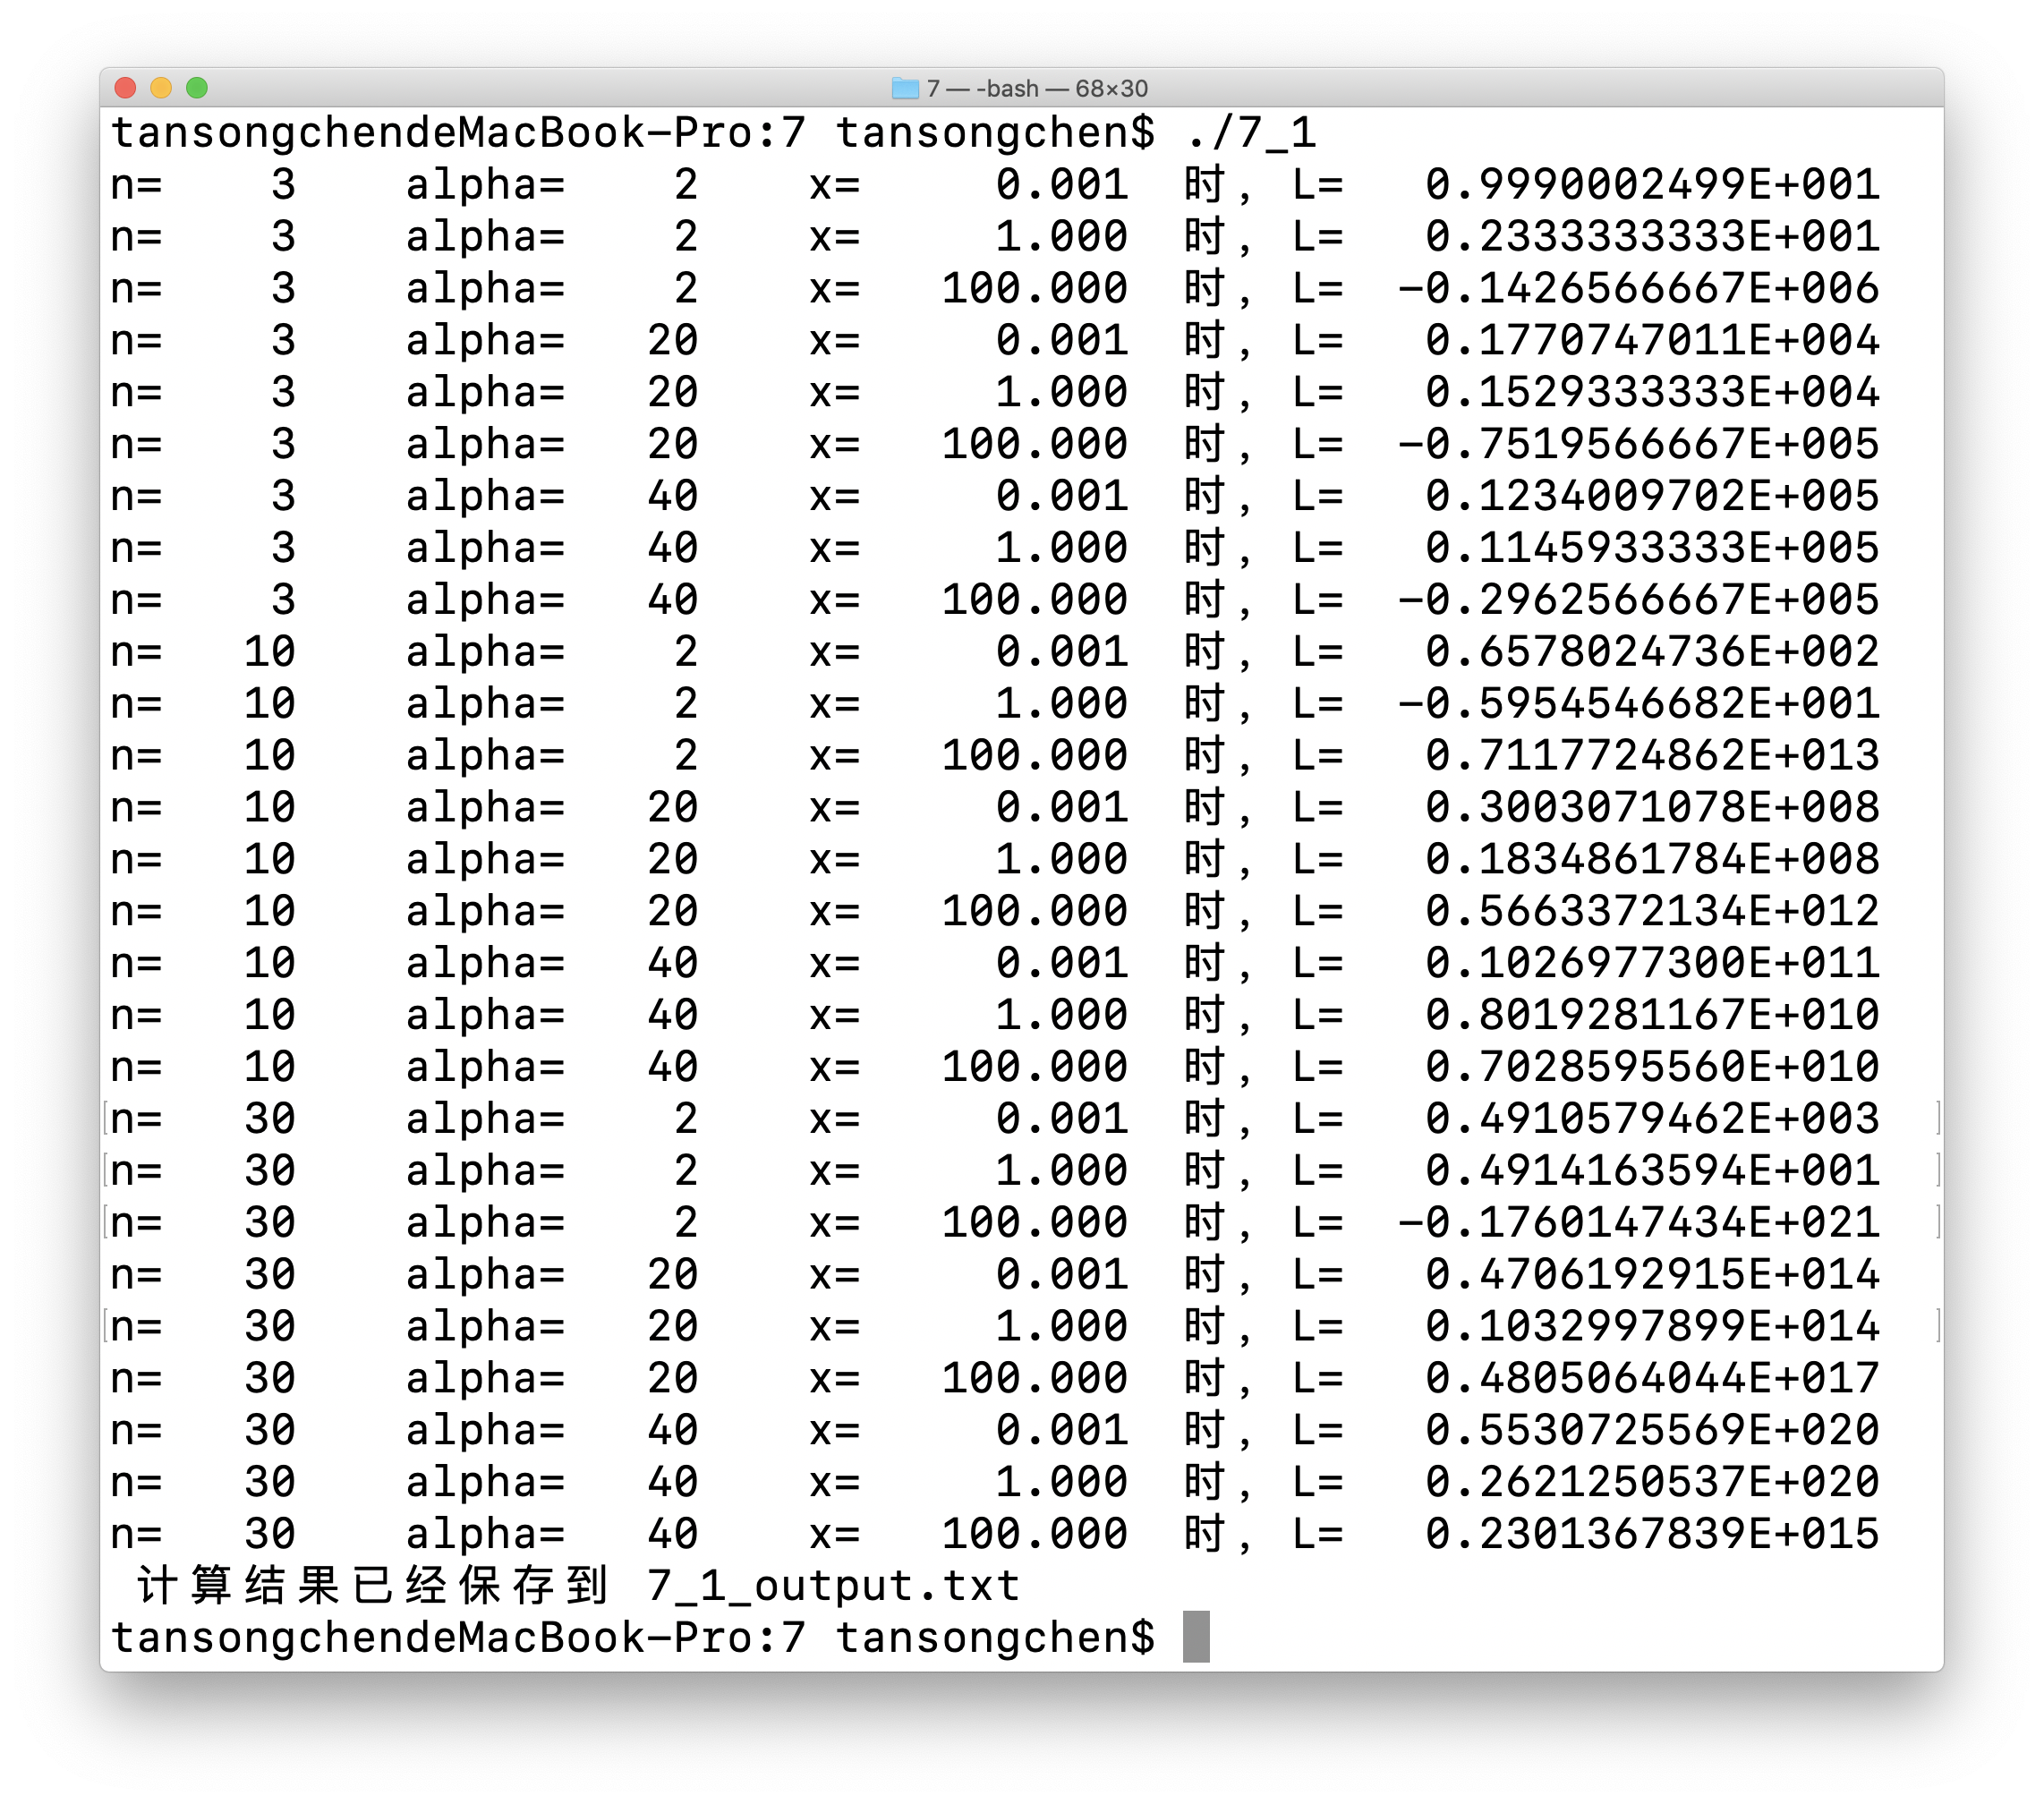
\includegraphics[scale = 0.3]{laguerre.png}
\caption{Laguerre 多项式求值}
\end{figure}
\subsection{源代码}
\begin{lstlisting}
program project7_1
	integer, parameter :: n(3) = (/3, 10, 30/)
	integer, parameter :: a(3) = (/2, 20, 40/)
	real*8 :: x(3) = (/0.001, 1.0, 100.0/)
	real*8, external :: L
	integer i, j, k
	real*8 output

	open (11, file = '7_1_output.txt')
	write (11, '(A10,A10,A10,A20)') &
	'n', 'alpha', 'x', 'L'
	do i=1,3
		do j=1,3
			do k=1,3
				! 遍历给定的几组参数,分别输出
				output = L(n(i),a(j),x(k))
				write (*, &
				'(A2,I5,A10,I5,A6,F10.3,A10,E20.10E3)') &
				'n=', n(i), 'alpha=', a(j), 'x=', x(k), &
				'时,L=', output
				write (11, '(I10,I10,F10.3,E20.10E3)') &
				n(i), a(j), x(k), output
			end do
		end do
	end do
	write (*, *) '计算结果已经保存到 7_1_output.txt'
end program

function L(n, a, x)
	integer n, a, i
	real*8 x, f, g, h, L
	! n = 0 和 n = 1 时的初值
	f = 1
	g = 1+a-x
	! 开始递推
	do i = 1, n-1
		h = (-(i+a)*f+(2*i+1+a-x)*g)/(i+1)
		f = g
		g = h
	end do
	L = g
	return
end function
\end{lstlisting}
\newpage
\section{球谐函数的递推求值}
\subsection{问题描述}
求球谐函数 $Y_{lm}(\theta,\phi)$ 在如下情况时的值:$l=100, 500, 1000; m=1, l/100, l/10, l-1;$ 而 $\theta=0.001\pi, 0.3\pi, 0.501\pi;\phi=0.4\pi$。
\subsection{解答思路}
定义约化连带 Legendre 函数将球谐函数可以表示为:
\[
Y_{lm}(\theta,\phi)=Q_l^m(\cos\theta)e^{im\phi}
\]

则该函数将满足如下的递推关系:

\[
Q_l^m(x)=x\sqrt{\frac{4l^2-1}{l^2-m^2}}Q_{l-1}^m(x)-\sqrt{\frac{2l+1}{2l-3}\frac{(l-1)^2-m^2}{l^2-m^2}}Q_{l-2}^m(x)
\]

从 $m=l$ 处开始递推,初始值为

\[
Q_m^m(x)=(-1)^m(1-x^2)^{m/2}\sqrt{\frac{(2m+1)!!}{4\pi(2m)!!}}
\]

计算该初始值时,注意到其中乘幂项为 $\sin^m\theta$,当 $m$ 特别大时该数会下溢。在计算前,取出其小数部分(在 0.5 到 1 之间),显然小数部分的 1000 次方大于 $2^{-1000}$,作为双精度数不会下溢,然后将指数部分乘以幂次即可;最后输出时,手动整理为十进制下的科学计数法输出。

我们形式地赋另一初值 $Q_{m-1}^m=0$,则利用如上线性递推公式从 $m+1$ 推到 $l$ 即可。

另外,当 $m$ 取 5, 10, 50, 100 时,球谐函数的虚部应为 0,但由于 $\pi$ 和三角函数的精度限制,算出并不为 0。此时为使该行为得到满足,强制将虚部置为 0。
\subsection{算法描述}
\begin{lstlisting}
输入:l, m, theta, phi = 0.4 pi
输出:Y

z = exp(i*m*phi)
! 当 m 是 5 的倍数时将 sin m*phi 强制置 0
if (m = 5k) Im(z) = 0

! 调用函数计算,分别用 fraction 和 exponent 表示指数和小数部分
x = cos(theta)
fraction, exponent = P(l, m, x)
Y = fraction * z
! 按科学计数法,将实部调整到 1 至 10 的范围内
if (abs(Re(Y)) < 1) then
    Y = Y * 10
    exponent = exponent - 1
write Y

function P(l, m, x)
    ! 取出数的指数和小数部分
    part_e = exponent(1-x**2)
    part_f = fraction(1-x**2)
    ! 先算 P_mm,归一化系数用 A 表示,代入 part_f 而不用原数值计算
    g = A * part_f ** (m/2.0)
    part_e = part_e * (m/2.0)
    ! 开始递推
    f = 0
    h = 0
    do i = m+1, l
        h = F(f, g) ! 递推关系
        f = g
        g = h
    ! 转至 10 进制表示
    g * 2**part_e → fraction * 10**exponent
    return (fraction, exponent)
end function
\end{lstlisting}
\subsection{计算结果及讨论}

\begin{figure}[h]
\centering
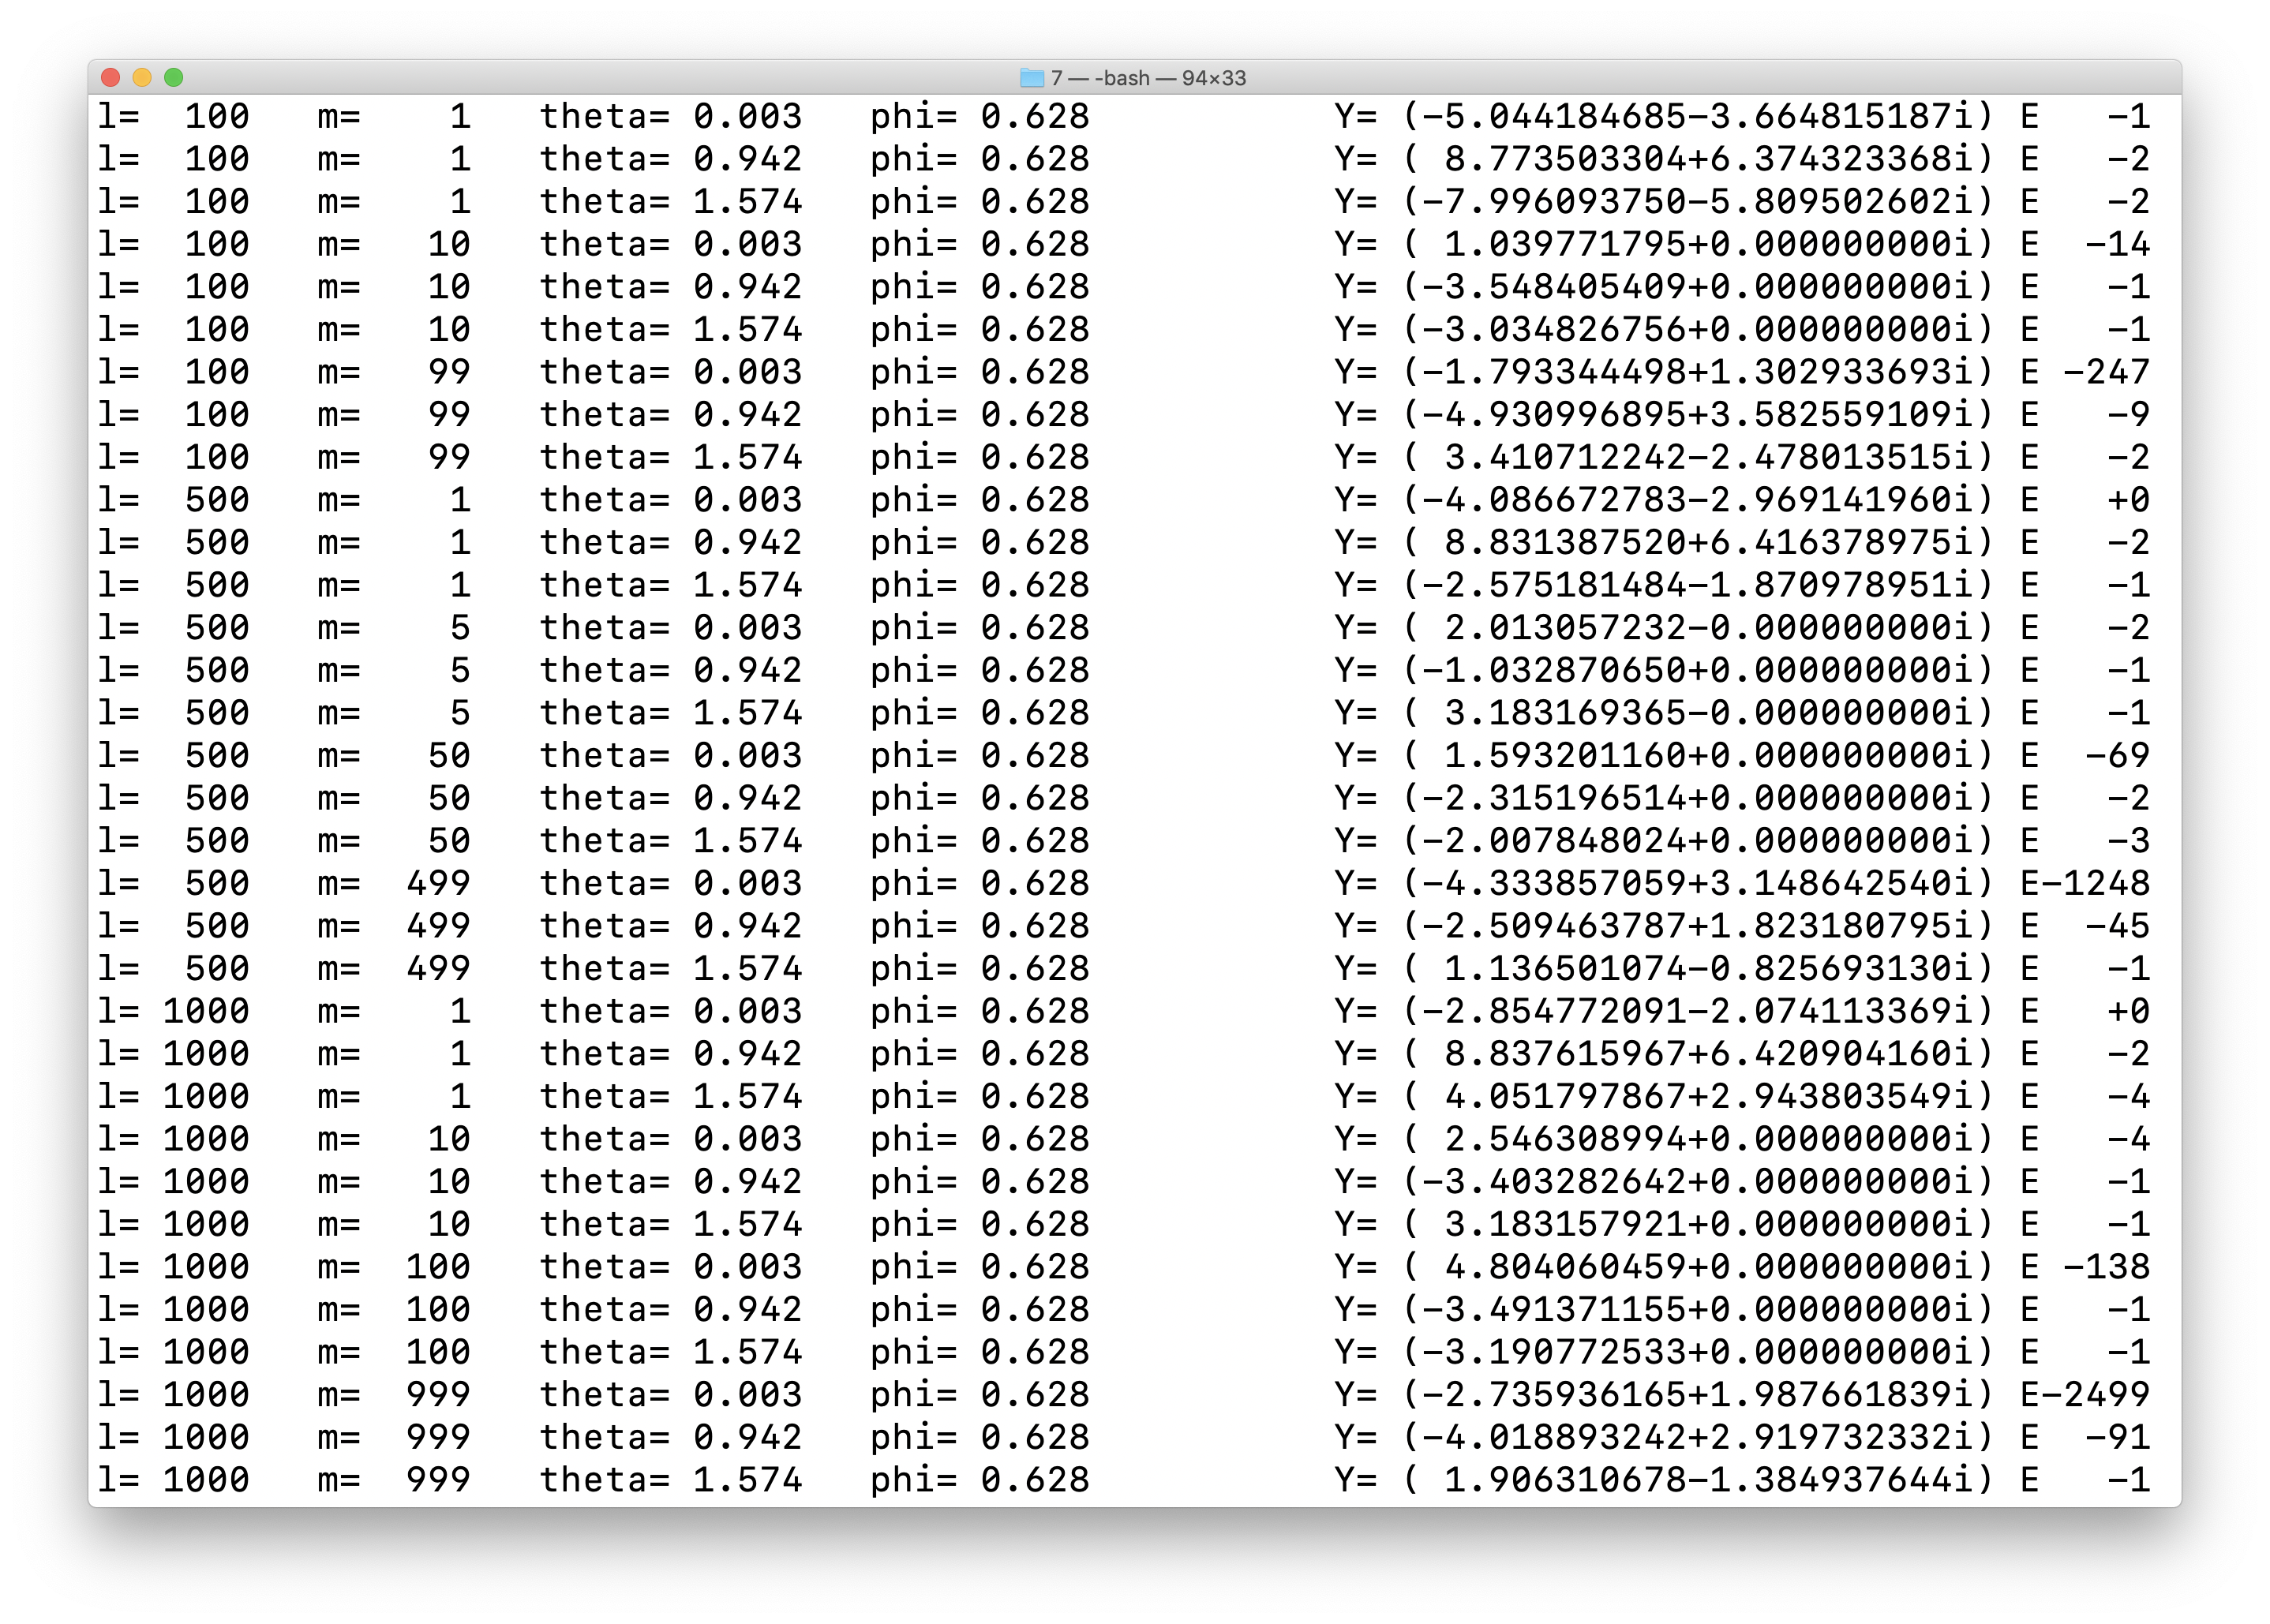
\includegraphics[scale = 0.27]{harmonics.png}
\caption{球谐函数求值}
\end{figure}

\subsection{源代码}
\begin{lstlisting}
program project7_2
	integer, parameter :: l(3) = (/100, 500, 1000/)
	integer :: i, j, k, m(4) = 0
	real*8, parameter :: pi = 3.14159265358979323846
	real*8, parameter :: theta(3) = (/0.001*pi, 0.3*pi, 0.501*pi/)
	real*8, parameter :: phi = pi*0.2
	! 先定义约化连带 Legendre 函数
	interface
		function P(l, m, x)
		integer l, m
		real*8 x, P(2)
		end function
	end interface
	complex*8 :: Y, z
	! 定义由指数和小数组成的数组,接收 P 函数的结果
	real*8 x, frac_exp(2), frac, exp

	open (11, file = '7_2_output.txt')
	write (11, '(A10,A10,A10,A10,A50)') &
	'l', 'm', 'theta', 'phi', 'Y'
	do i=1,3
		m = (/1, l(i)/100, l(i)/10, l(i)-1/)
		do j=1,4
			z = complex(cos(m(j) * phi), sin(m(j) * phi))
			! 修正由三角函数精确度不够造成的问题
			if (mod(m(j), 5) == 0) &
			z = complex(cos(m(j) * phi), 0)
			do k=1,3
				x = cos(theta(k))
				frac_exp = P(l(i),m(j),x)
				! 分别取出小数和指数部分
				frac = frac_exp(1)
				exp = frac_exp(2)
				Y = frac * z
				! 规范化科学计数法表示
				if (abs(real(Y)) < 1) then
					Y = Y * 10
					exp = exp - 1
				end if
				write (*, &
				'(A2,I5,A5,I5,A9,F6.3,A7,F6.3,$)') &
				'l=', l(i), 'm=', m(j), &
				'theta=', theta(k), 'phi=', phi
				write (*, '(A15,F12.9,SPF12.9,A4,I5)') &
				'Y= (', real(Y), aimag(Y), 'i) E', &
				floor(exp)
				write (11, '(I10,I10,F10.6,F10.6,$)') &
				l(i), m(j), theta(k), phi
				write (11, '(A5,F20.15,F20.15,A4,I5)') &
				'(', real(Y), aimag(Y), 'i) E', floor(exp)
			end do
		end do
	end do
	write (*, *) '计算结果已经保存到 7_2_output.txt'
end program

function P(l, m, x)
	integer l, m, i
	real*8, parameter :: pi = 3.14159265358979323846
	real*8 x, f, g, h, part_e, part_f, P(2), exp, exp_int
	part_e = exponent(1-x**2)
	part_f = fraction(1-x**2)
	! 先算 P_mm
	g = 1.0/4.0/pi
	do i = 1, m
		g = g*(2*i+1.0)/(2.0*i)
	end do
	g = sqrt(g) * (-1)**m * part_f**(m/2.0)
	! 开始递推
	f = 0
	h = 0
	do i = m+1, l
		h = x * sqrt((4 * i**2 - 1.0)/(i**2 - m**2)) * g - &
		sqrt(((i - 1)**2 - m**2)*(2 * i + 1.0)/ &
		(i**2 - m**2)/(2 * i - 3)) * f
		f = g
		g = h
	end do
	! 通过对数将以 2 为底的指数变成以 10 为底
	part_e = part_e * m / 2.0 + exponent(g)
	exp = part_e * log10(2.0)
	! 多余的部分乘到小数上,此时小数在 0.5 到 10 之间
	g = fraction(g) * 10 ** (exp - floor(exp))
	P = (/g, exp/)
	return
end function
\end{lstlisting}
\begin{figure}[h]
\centering
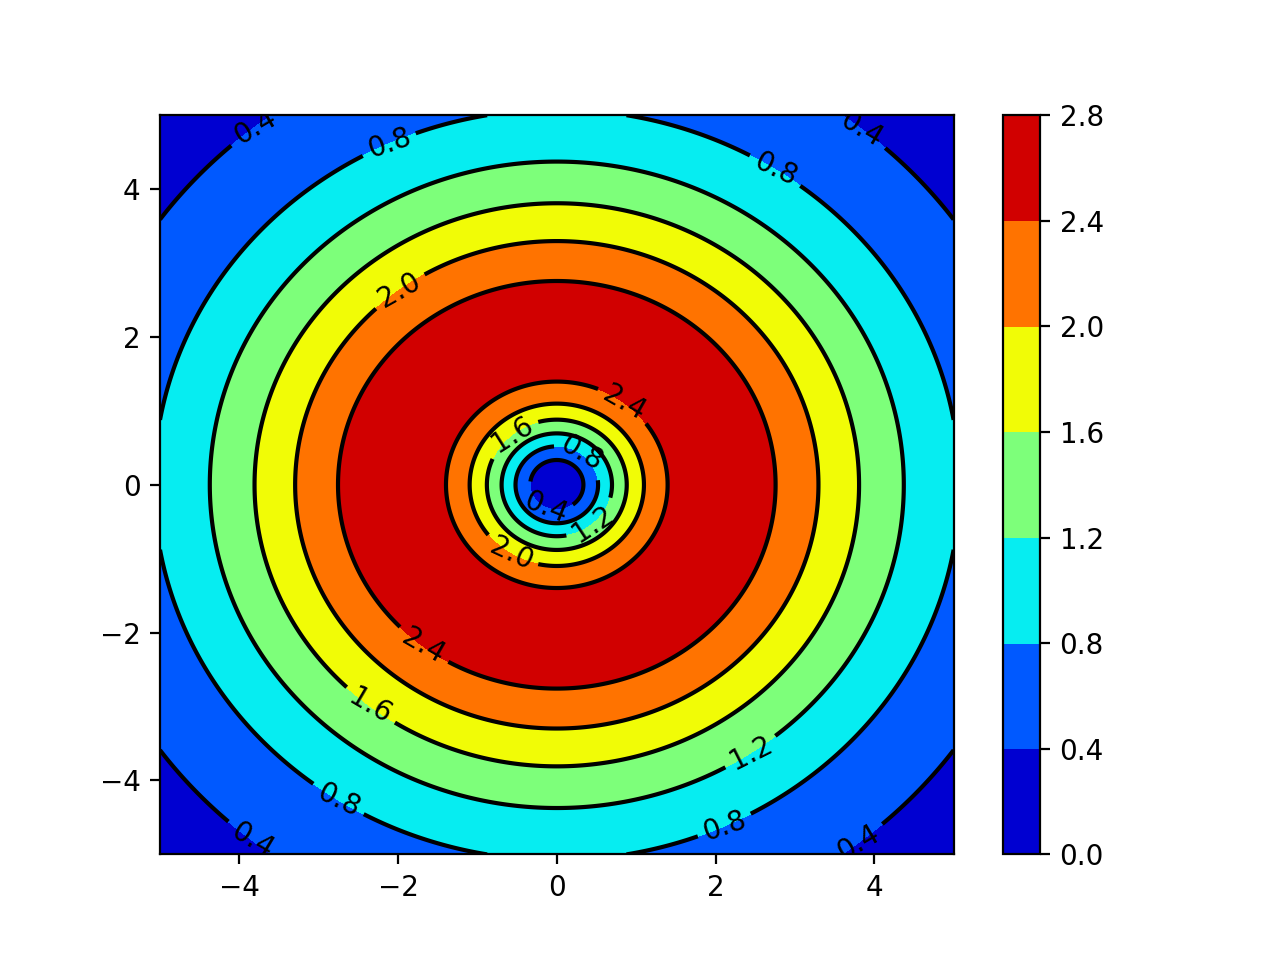
\includegraphics[scale = 0.8]{r11.png}
\caption{波函数取 $n=2, l=1, m=\pm1$ 时在 $z=0$ 平面上的概率分布图}
\end{figure}
\subsection{波函数作图}
首先代入 $n=2, l=1, \theta=\pi/2$ 推导 $\rho_{21m}$ 的形式:

\[
\rho_{21m}=\frac{e^{-r}r^2}{24}|Y_{1m}|^2
\]

代入 $m$,并在 $x-y$ 平面上转换为直角坐标形式,得到

\[
\rho_{211}=\rho_{21-1}=\frac{e^{-r}r^2}{64\pi}\sin^2\theta=\frac{e^{-\sqrt{x^2+y^2}}(x^2+y^2)}{64\pi}
\]

\[
\rho_{210}=\frac{e^{-r}r^2}{32\pi}\cos^2\theta= 0
\]

对 $\rho_{21\pm1}$ 选取 $|x|<5, |y|<5$ 作图(为便于显示等高线,将其中数据放大 $10^3$ 倍)。由此可以看出,对于 $2p_x,2p_y$ 轨道,$z=0$ 平面上的分布仅与 $r$ 有关,而与 $\phi$ 无关;对于 $2p_z$ 轨道,$z=0$ 平面上没有电子出现的概率。

\newpage

\section{氢原子能量计算}
\subsection{问题描述}
计算 $n=3,l=1,m=1$ 时氢原子能量 $E=\langle\Psi|H|\Psi\rangle$,要求误差不大于 $10^{-6}$。
\subsection{解答思路}
在该条件下,波函数为
\[
\frac1{81\sqrt \pi}r(r-6)e^{-r/3}\sin\theta e^{i\phi}
\]

记径向波函数为 R,则能量本征值可以表示为:

\[
\frac1{6561\pi}\int_0^\infty\int_0^\pi\int_0^{2\pi} R(r)\sin\theta e^{-i\phi}\times\left[-\frac12\left(\frac1{r^2}\frac{\partial}{\partial r}(r^2\frac{\partial}{\partial r})-\frac2{r^2}\right)-\frac1r\right]\times R(r)\sin\theta e^{-i\phi}\times r^2\sin\theta \f r\f\theta\f\phi
\]

于是可以先求出角度部分积分(含有系数):
\[
\frac1{6561\pi}\int_{0}^{\pi}\sin^3\theta d\theta\int_0^{2\pi}d\phi=\frac{8}{19683}
\]

利用(变换使差分计算方便)

\[
\frac1{r^2}\frac{\partial}{\partial r}(r^2\frac{\partial}{\partial r})=\frac1r\frac{\partial^2}{\partial r^2}r
\]

剩余部分可以表为

\[
-\int_0^\infty R(r)\times\left[\frac12(rR(r))''+(r-1)R(r)\right]\f r
\]

于是,我们先在 [0, 60] 上取一定数量的点计算出 $R(r)$,然后计算出 $rR(r)$,利用二阶导数的有限差分近似得到积分中的导数项,然后再进行数值积分即可求得。
\subsection{算法描述}
\begin{lstlisting}
输入:step = 0.01, count = 6000
输出:integral

r = (step*i, 0<= i <= count+1)
! 计算 R、rR
forall (i=0:(count+1))
    R(i) = f(r(i))
    rR(i) = r(i)*R(i)
! 计算 rR 的二阶导数
forall (i=1:count)
    ddrR(i) = (rR(i+1) + rR(i-1) - 2*rR(i))/step**2
! 计算积分
do i = 1, count
    integral = integral + F(r(i)) * step
! 乘上角度部分系数
integral = integral * (-8) / 19683
write integral
\end{lstlisting}
\subsection{计算结果及讨论}
\begin{figure}[h]
\centering
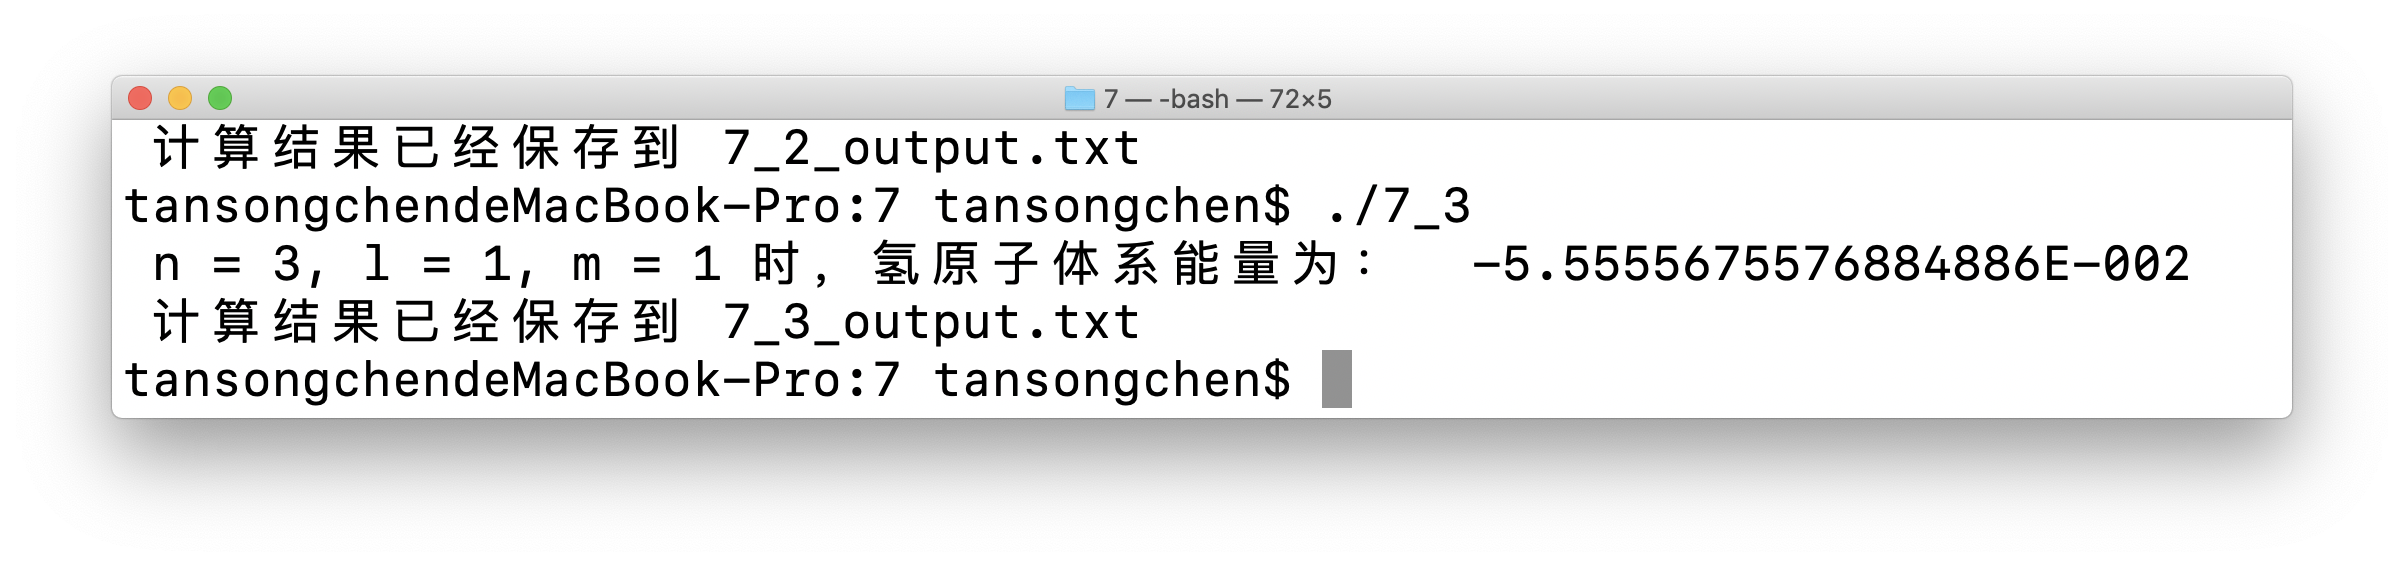
\includegraphics[scale = 0.3]{hydrogen.png}
\caption{氢原子能量计算}
\end{figure}
精确解为 $0.55555...$,计算误差约为 $1.2\times 10^{-7}$。考虑到数值微分和积分以 $O(h^2)$ 收敛,还能够进一步增加步长以减小计算量。

另尝试,若先解析算出微分,再进行积分,则取步长为 0.1 时即能满足精度要求。
\subsection{源代码}
\begin{lstlisting}
program project7_3
	real*8, parameter :: limit = 60.0, step = 0.01
	integer, parameter :: count = nint(limit/step)
	real*8, parameter :: r_sample(0:count+1) = &
	(/(i*step, i=0, count+1)/)
	real*8 :: integral = 0.0
	real*8 R(0:count+1), rR(0:count+1), ddrR(1:count)
	integer i

	open (11, file = '7_3_output.txt')
	! 计算 R
	forall (i=0:(count+1)) R(i) = r_sample(i)*(r_sample(i)-6) * &
	                              exp(-r_sample(i)/3)
	! 计算 rR
	rR = r_sample*R
	! 计算 rR 的二阶导数
	forall (i=1:count) ddrR(i) = (rR(i+1) + rR(i-1) - 2*rR(i))/step**2
	! 计算积分
	do i = 1, count
		integral = integral + R(i) * (r_sample(i)*0.5*ddrR(i) + &
			       (r_sample(i)-1)*R(i)) * step
	end do
	! 乘上角度部分系数
	integral = integral * (-8) / 19683
	write (*, *) 'n = 3, l = 1, m = 1 时,氢原子体系能量为:', integral
	write (11, *) integral
	write (*, *) '计算结果已经保存到 7_3_output.txt'
end program
\end{lstlisting}
\newpage
\appendix
\section{致谢}
感谢北京大学物理学院彭良友老师对于计算物理学知识详尽准确的介绍。

感谢北京大学物理学院赵忠海学长、刘士琦学姐针对作业进行的必要的提示以及回答我在编写程序时的疑问。

感谢北京大学化学与分子工程学院张志钧学长在有关 Fortran 编译的问题上回答我的疑问。
\end{document}